\documentclass{article}%
\usepackage[T1]{fontenc}%
\usepackage[utf8]{inputenc}%
\usepackage{lmodern}%
\usepackage{textcomp}%
\usepackage{lastpage}%
%
\usepackage{amsmath}%
\usepackage{amssymb}%
\usepackage{amsfonts}%
\usepackage{graphicx}%
\usepackage{hyperref}%
\usepackage{tikz}%
\usepackage{pgfplots}%
\usetikzlibrary{math}%
\title{ITA 2026 - Física\thanks{This exam was solved and automatically generated with gpt-resolve: \url{https://github.com/lgabs/gpt-resolve}}}%
\author{claude{-}haiku{-}5{-}5 (solver) + claude{-}haiku{-}5{-}5 (judge)}%
\date{November 10, 2026}%
%
\begin{document}%
\normalsize%
\maketitle%
\section*{Questão 1}

\section*{Solução}

\textbf{Hipóteses, figura e convenções.}
\begin{itemize}
\item (i) Trilhos horizontais e $v$ constante: a aceleração do trem é só centrípeta. Como $R$ é muito maior que o trem, todas as rodas têm o mesmo centro de curvatura $C$, situado na direção do eixo. A força centrípeta $F=\dfrac{Mv^2}{R}$ é horizontal e dirigida a $C$. O trem é tratado como corpo rígido sobre o eixo, e o equilíbrio global vale para qualquer número de rodas. O tombamento não é considerado, pois a altura do centro de massa não é dada; um trem real pode ter restrição adicional de torque, o que é uma limitação do modelo.
\item (ii) Pela figura, a face de maior raio de cada roda está voltada para o eixo, a geratriz inferior sobe para fora e o trilho apoia-se nela. Logo a normal de contato de cada roda aponta para cima e para o centro do eixo, inclinada de $\theta$ com a vertical. Chamo $E$ a roda externa (mais afastada de $C$) e $I$ a interna.
\item (iii) O trilho só empurra: $N_w\ge 0$, e perder o contato significa $N_w=0$. O atrito estático obedece a $|f_w|\le\mu N_w$.
\item (iv) O atrito longitudinal (na direção dos trilhos) é nulo: as rodas rolam livres, sem tração nem frenagem. Se existisse, ele reduziria a componente transversal disponível ($f_t^2+f_\ell^2\le\mu^2N^2$), só piorando a situação. As cotas abaixo, atingidas com $f_\ell=0$, continuam válidas.
\end{itemize}

\textbf{Equações.} Uso $H$ horizontal (positivo para $C$) e $V$ vertical (positivo para cima). A reação de cada roda é $\vec R_w=N_w\vec n_w+f_w\vec t_w$, com $\vec n_w$ a normal e $\vec t_w$ a geratriz inferior. Tomo $f_w>0$ quando a componente horizontal do atrito aponta para $C$:
\[
\vec R_E=N_E(\sin\theta,\ \cos\theta)+f_E(\cos\theta,\ -\sin\theta),\qquad
\vec R_I=N_I(-\sin\theta,\ \cos\theta)+f_I(\cos\theta,\ \sin\theta).
\]
O equilíbrio do trem dá
\[
\sum_w H_w=\frac{Mv^2}{R},\qquad \sum_w V_w=Mg.
\]

\textbf{b) Atrito desprezível.} Com $f_E=f_I=0$:
\[
(N_E-N_I)\sin\theta=\frac{Mv^2}{R},\qquad (N_E+N_I)\cos\theta=Mg,
\]
e, portanto,
\[
N_I=\frac12\left(\frac{Mg}{\cos\theta}-\frac{Mv^2}{R\sin\theta}\right).
\]
Quando $R$ diminui, $N_I$ diminui: a roda interna é a que se levanta. $N_I\ge 0$ equivale a $\dfrac{v^2}{R}\le g\tan\theta$. No limiar $N_I=0$ e
\[
R_{\min}=\frac{v^2}{g\tan\theta}.
\]

\textbf{a) Atrito $\mu$.} Seja $\varphi=\arctan\mu$, com $0<\theta<90^\circ$. Suponho $\mu\tan\theta<1$, isto é, $\theta+\varphi<90^\circ$. O caso contrário é tratado no fim.

\emph{Passo 1 (configuração limite).} Impondo $N_I=0$, $f_I=0$ e $f_E=\mu N_E$ (roda interna prestes a levantar, roda externa no limite de atrito), as equações de equilíbrio dão
\[
N_E(\cos\theta-\mu\sin\theta)=Mg,\qquad N_E(\sin\theta+\mu\cos\theta)=\frac{Mv^2}{R}.
\]
Com $\mu\tan\theta<1$, $N_E=\dfrac{Mg}{\cos\theta-\mu\sin\theta}>0$. Dividindo uma equação pela outra,
\[
\frac{v^2}{gR}=\frac{\sin\theta+\mu\cos\theta}{\cos\theta-\mu\sin\theta}=\frac{\tan\theta+\mu}{1-\mu\tan\theta}=\tan(\theta+\varphi).
\]

\emph{Passo 2 (nenhum equilíbrio admissível para $R<R_{\min}$).} Escrevo $f_w=N_w\tan\beta_w$, com $|\beta_w|\le\varphi$ por causa de $|f_w|\le\mu N_w$. Seja $\psi_w$ o ângulo de $\vec R_w$ com a vertical, positivo para $C$. Então
\[
\tan\psi_E=\frac{N_E\sin\theta+f_E\cos\theta}{N_E\cos\theta-f_E\sin\theta}=\tan(\theta+\beta_E),\qquad
\tan\psi_I=\frac{-N_I\sin\theta+f_I\cos\theta}{N_I\cos\theta+f_I\sin\theta}=\tan(\beta_I-\theta),
\]
donde $\psi_E\in[\theta-\varphi,\ \theta+\varphi]$ e $\psi_I\in[-\theta-\varphi,\ \varphi-\theta]$. Em ambos os casos $|\psi_w|\le\theta+\varphi<90^\circ$. Logo $V_w\ge 0$ e $H_w=V_w\tan\psi_w\le V_w\tan(\theta+\varphi)$. Somando sobre as rodas,
\[
\frac{Mv^2}{R}=\sum_w H_w\le\tan(\theta+\varphi)\sum_w V_w=Mg\tan(\theta+\varphi)\quad\Longrightarrow\quad R\ge R_{\min}.
\]
Logo o passo 1 dá o máximo de $\sum H$, e para $R<R_{\min}$ não há equilíbrio com contato e sem deslizamento.

\emph{Passo 3 (existência para $R>R_{\min}$).} As configurações $(N_w,f_w)$ com $N_w\ge 0$, $|f_w|\le\mu N_w$ e $\sum V_w=Mg$ formam um conjunto convexo. Dois de seus pontos são $P_0$, com $N_E=N_I=\dfrac{Mg}{2\cos\theta}$ e $f_w=0$ (então $\sum H=0$), e $P^*$ do passo 1 (com $\sum H=Mg\tan(\theta+\varphi)$). Para $R>R_{\min}$ tem-se $F=\dfrac{Mv^2}{R}\in\bigl(0,\,Mg\tan(\theta+\varphi)\bigr)$. A combinação $\lambda P^*+(1-\lambda)P_0$, com $\lambda=F/[Mg\tan(\theta+\varphi)]\in(0,1)$, é admissível, tem $\sum H=F$ e $N_E,N_I>0$. Assim as duas rodas permanecem em contato. Em $P^*$ o atrito na roda externa aponta para $C$ e para baixo, sentido que se opõe à tendência de o trem escorregar para fora da curva.

\emph{Caso $\mu\tan\theta\ge 1$.} Agora $\theta+\varphi\ge 90^\circ$ e o passo 2 deixa de valer: $\psi_E$ pode ultrapassar $90^\circ$, isto é, $V_E<0$. Com os dois atritos no limite,
\[
\vec R_E=s\,\bigl(\sin(\theta+\varphi),\cos(\theta+\varphi)\bigr),\qquad \vec R_I=u\,\bigl(\sin(\varphi-\theta),\cos(\varphi-\theta)\bigr),\qquad s\ge 0,
\]
com $u=\dfrac{Mg-s\cos(\theta+\varphi)}{\cos(\varphi-\theta)}\ge 0$, pois $\cos(\theta+\varphi)\le 0<\cos(\varphi-\theta)$. Então
\[
\sum H=Mg\tan(\varphi-\theta)+\frac{s\sin 2\theta}{\cos(\varphi-\theta)}\longrightarrow\infty\quad (s\to\infty).
\]
Dentro do modelo de Coulomb há equilíbrio sem perda de contato para todo $R>0$. Esse resultado é um artefato: o trilho ``crava'' a roda externa (efeito de cunha, com força para baixo de módulo arbitrário), o que exige forças de contato ilimitadas e indeterminadas pela estática de corpo rígido. Na prática, a deformação e a resistência dos materiais limitam essas forças. Portanto, nesse regime a estática não fornece cota inferior útil: $R_{\min}=0$ só no modelo, e a hipótese de corpo rígido deixa de valer.

\textbf{c) Rodas cilíndricas.} Com $\theta=0$, a normal é vertical e o atrito é horizontal:
\[
\sum_w N_w=Mg,\qquad \sum_w f_w=\frac{Mv^2}{R},\qquad |f_w|\le\mu N_w.
\]
Logo $\dfrac{Mv^2}{R}\le\mu\sum_w N_w=\mu Mg$, ou seja, $R\ge \dfrac{v^2}{\mu g}$. A desigualdade vale também com atrito longitudinal, pois $|f_t|\le\mu N$. A igualdade ocorre com $f_w=\mu N_w$ voltado para $C$ nas duas rodas, para qualquer repartição $N_E+N_I=Mg$ com $N_E,N_I>0$ (por exemplo, $N_E=N_I=\dfrac{Mg}{2}$). Aqui o limite é o atrito, não o contato: a carga se reparte com normais positivas, e nenhuma roda perde contato para qualquer $R$.

\textbf{Checagens.}
\begin{itemize}
\item Unidades: $\dfrac{v^2}{g}$ tem dimensão de metro, e as tangentes são adimensionais.
\item Limites: em (a), $\mu\to 0$ recupera (b) e $\theta\to 0$ recupera (c). Em (b), $\theta\to 0$ dá $R\to\infty$ (cilindros lisos não curvam) e $\theta\to 90^\circ$ dá $R\to 0$.
\item Para $\theta+\varphi<90^\circ$ vale $\tan(\theta+\varphi)\ge\max(\tan\theta,\mu)$, logo $R_{(a)}\le\min(R_{(b)},R_{(c)})$: a inclinação do cone e o atrito somam-se para sustentar a curva.
\item Numérico: $v=30\ \text{m/s}$, $\theta=45^\circ$, $\mu=0{,}3$: $R_{(a)}=\dfrac{900\cdot 0{,}7}{10\cdot 1{,}3}\approx 48{,}5\ \text{m}$, $R_{(b)}=90\ \text{m}$, $R_{(c)}=300\ \text{m}$.
\item Ordem de grandeza: com $\tan\theta=0{,}05$ (conicidade $1/20$) e $\mu=0{,}3$, $R_{(a)}=\dfrac{v^2(1-0{,}015)}{0{,}35\,g}\approx 2{,}8\,\dfrac{v^2}{g}\approx 250\ \text{m}$ para $v=30\ \text{m/s}$ (cerca de $108$ km/h).
\end{itemize}

ANSWER: (a) $R_{\min}=\dfrac{v^2}{g\tan(\theta+\arctan\mu)}=\dfrac{v^2(1-\mu\tan\theta)}{g(\mu+\tan\theta)}$ para $\mu\tan\theta<1$ (para $\mu\tan\theta\ge 1$ não há cota inferior no modelo); (b) $R_{\min}=\dfrac{v^2}{g\tan\theta}$; (c) $R_{\min}=\dfrac{v^2}{\mu g}$.%
\newpage%
\section*{Questão 2}

\section*{Solução}

\textbf{Hipóteses.}
\begin{enumerate}
\item Equilíbrio estático do corpo rígido. A figura mostra a barra elevada sobre os suportes, mas o enunciado não fornece essa altura nem a geometria dos apoios. Por isso idealiza-se a linha de centro da barra e os contatos como situados sobre a superfície do plano, de modo que todas as forças atuam nessa linha. Essa idealização é obrigatória: se a linha das cargas estivesse a uma altura $\delta$ acima dos contatos, os momentos das componentes dos pesos paralelas ao plano alterariam $N_A$ e $N_B$ em sentidos opostos, de $\pm\,\delta\,g\sin\theta\,(M+m+m_c)/(L-2d)$. No exemplo numérico abaixo, $\delta=1$ cm já causaria uma variação de cerca de $0{,}4$ N, e $\delta$ não é dado.
\item Contatos pontuais em $A$ e $B$, com $d<L/2$, logo $L-2d>0$.
\item Pesos são forças concentradas: $Mg$ no centro da barra (homogênea), $mg$ em $s=a$ e $m_cg$ em $s=L-b$.
\item Os apoios só empurram ($N_A\ge 0$, $N_B\ge 0$), e o atrito é estático.
\end{enumerate}

\textbf{Referencial e forças sobre a barra.} Seja $s$ a posição ao longo da barra, medida a partir da extremidade inferior. Use os versores $\hat e_s=(\cos\theta,\sin\theta)$, ao longo do plano para cima, e $\hat e_n=(-\sin\theta,\cos\theta)$, normal ao plano para fora, nas coordenadas (horizontal, vertical). Então $(0,1)=\sin\theta\,\hat e_s+\cos\theta\,\hat e_n$, e cada peso $-m_i g\,(0,1)$ tem componentes $-m_i g\sin\theta$ em $\hat e_s$ e $-m_i g\cos\theta$ em $\hat e_n$. As forças que os apoios exercem sobre a barra são $N_A\hat e_n+f_A\hat e_s$ em $s=d$ e $N_B\hat e_n+f_B\hat e_s$ em $s=L-d$. Pela 3ª lei, a barra comprime os apoios com forças de módulos $N_A$ e $N_B$, para dentro do plano, e os atritos sobre os apoios apontam no sentido descendente do plano.

\textbf{Equações de equilíbrio.} Resultantes nas direções $\hat e_n$ e $\hat e_s$:
\[
N_A+N_B=(M+m+m_c)\,g\cos\theta \tag{1}
\]
\[
f_A+f_B=(M+m+m_c)\,g\sin\theta \tag{2}
\]
Momentos em torno de um eixo perpendicular ao plano $\Pi$ da barra e passando por um ponto $s_0$: a força $F_n\hat e_n$ aplicada em $s$ tem momento $(s-s_0)F_n$, enquanto $F_s\hat e_s$ tem momento nulo, pois atua ao longo da própria linha da barra, que contém o eixo. Assim, os atritos e as componentes $-m_i g\sin\theta$ dos pesos não contribuem. Em torno de $A$ e de $B$:
\[
N_B\,(L-2d)=g\cos\theta\Big[M\big(\tfrac{L}{2}-d\big)+m\,(a-d)+m_c\,(L-b-d)\Big] \tag{3}
\]
\[
N_A\,(L-2d)=g\cos\theta\Big[M\big(\tfrac{L}{2}-d\big)+m\,(L-a-d)+m_c\,(b-d)\Big] \tag{4}
\]
Há quatro incógnitas ($N_A$, $N_B$, $f_A$, $f_B$), mas só três equações independentes: (4) decorre de (1) e (3).

\textbf{Item a).} Cada normal sai de uma única equação de momentos, o que é a regra da alavanca:
\[
N_A=\frac{g\cos\theta}{L-2d}\Big[M\big(\tfrac{L}{2}-d\big)+m\,(L-a-d)+m_c\,(b-d)\Big]
\]
\[
N_B=\frac{g\cos\theta}{L-2d}\Big[M\big(\tfrac{L}{2}-d\big)+m\,(a-d)+m_c\,(L-b-d)\Big]
\]
Conferências algébricas (não são equações físicas novas). (i) Como $(L-a-d)+(a-d)=L-2d$ e $(b-d)+(L-b-d)=L-2d$, a soma das expressões reproduz (1). (ii) O momento em torno do centro da barra, ponto distinto de $A$ e $B$, deve satisfazer $(N_B-N_A)(L/2-d)=g\cos\theta\,[m(a-L/2)+m_c(L/2-b)]$; substituindo as expressões acima, a igualdade se verifica.

\textbf{Item b).} Por (2), a estática fixa apenas a soma $f_A+f_B$. Como há uma incógnita a mais que as equações independentes, a repartição entre $A$ e $B$ depende da deformação dos contatos, que o enunciado não fornece. Adota-se, como hipótese explícita, a mobilização uniforme do atrito: a razão entre atrito e normal é a mesma nos dois apoios,
\[
\frac{f_A}{N_A}=\frac{f_B}{N_B}=\mu_m .
\]
Sentido físico: cada apoio mobiliza a mesma fração de atrito em relação à sua carga normal, análogo à hipótese de mobilização uniforme da resistência ao cisalhamento usada em análises de estabilidade de taludes. Equivalentemente, a reação de contato em cada apoio forma com a normal ao plano o ângulo $\arctan\mu_m$. Com (1) e (2), $\mu_m(N_A+N_B)=(M+m+m_c)\,g\sin\theta$ e $N_A+N_B=(M+m+m_c)\,g\cos\theta$, logo $\mu_m=\tan\theta$. Portanto
\[
f_A=N_A\tan\theta=\frac{g\sin\theta}{L-2d}\Big[M\big(\tfrac{L}{2}-d\big)+m\,(L-a-d)+m_c\,(b-d)\Big]
\]
\[
f_B=N_B\tan\theta=\frac{g\sin\theta}{L-2d}\Big[M\big(\tfrac{L}{2}-d\big)+m\,(a-d)+m_c\,(L-b-d)\Big]
\]
Verificação: $N_A\hat e_n+f_A\hat e_s=\dfrac{N_A}{\cos\theta}(0,1)$, pois $\hat e_n+\tan\theta\,\hat e_s=(0,1/\cos\theta)$. Assim, a reação em cada apoio é vertical, com módulo $N_i/\cos\theta$. Ambas as frações são positivas, pois o atrito atua para cima do plano, opondo-se à tendência de descida.

Esse fechamento não decorre da estática. Outras repartições também satisfazem (2); por exemplo, $f_A=f_B$ corresponderia a contatos idênticos e elásticos com a barra transladando sem girar no plano. O total $(M+m+m_c)\,g\sin\theta$ independe do modelo; apenas as parcelas individuais dependem dele.

\textbf{Validade.}
\begin{itemize}
\item Atrito: com o fechamento, $|f_i|\le\mu_i N_i$ exige $\mu_i\ge\tan\theta$ em cada apoio. Para qualquer repartição, $f_A+f_B\le\mu_A N_A+\mu_B N_B$ exige $\tan\theta\le(\mu_A N_A+\mu_B N_B)/(N_A+N_B)$; com $\mu_A=\mu_B=\mu_s$, isso se reduz a $\mu_s\ge\tan\theta$.
\item Contato: $N_A\ge 0$ e $N_B\ge 0$, ou seja, os colchetes de (a) são não negativos. Se um deles for negativo, o apoio correspondente deveria puxar a barra; a barra então se descola dele e o modelo deixa de valer.
\item Caso degenerado $L=2d$: os apoios coincidem no centro, (3) e (4) reduzem-se a condições sobre as cargas ($0=g\cos\theta\,[\dots]$), e apenas $N_A+N_B$ fica determinado. Por isso as fórmulas exigem $L>2d$.
\end{itemize}

\textbf{Casos particulares.} Se $m=m_c=0$, então $N_A=N_B=\dfrac{Mg\cos\theta}{2}$ e $f_A=f_B=\dfrac{Mg\sin\theta}{2}$. Se $a=d$ e $m_c=0$, então $N_A=g\cos\theta\left(\dfrac{M}{2}+m\right)$ e $N_B=\dfrac{Mg\cos\theta}{2}$: toda a carga de $m$ vai para $A$. Se $a=L/2$ e $m_c=0$, então $N_A=N_B=\dfrac{(M+m)g\cos\theta}{2}$. Se $\theta=0$, os atritos se anulam e as normais somam o peso total.

\textbf{Unidades.} $g$ em m/s$^2$ vezes massa em kg dá newtons. O quociente $(L-a-d)/(L-2d)$ é adimensional, de modo que cada termo entre colchetes tem unidade de massa, e $N_i$ e $f_i$ saem em newtons.

\textbf{Exemplo numérico.} Com $M=10$ kg, $m=2$ kg, $m_c=1$ kg, $L=2$ m, $d=0{,}2$ m, $a=0{,}6$ m, $b=0{,}5$ m e $\theta=30^\circ$, obtém-se $N_A\approx 57{,}9$ N, $N_B\approx 54{,}7$ N, $f_A\approx 33{,}4$ N e $f_B\approx 31{,}6$ N. Conferências: $N_A+N_B\approx 112{,}6$ N $\approx 130\cos 30^\circ$ N; $f_A+f_B\approx 65{,}0$ N $=130\sin 30^\circ$ N, com $(M+m+m_c)g=130$ N; é preciso $\mu_s\ge\tan 30^\circ\approx 0{,}58$. Ordem de grandeza: peso total de 130 N, com cerca de 55 a 58 N em cada apoio.

ANSWER: a) $N_A=\dfrac{g\cos\theta}{L-2d}\left[M\left(\frac{L}{2}-d\right)+m\,(L-a-d)+m_c\,(b-d)\right]$ e $N_B=\dfrac{g\cos\theta}{L-2d}\left[M\left(\frac{L}{2}-d\right)+m\,(a-d)+m_c\,(L-b-d)\right]$; b) $f_A=N_A\tan\theta=\dfrac{g\sin\theta}{L-2d}\left[M\left(\frac{L}{2}-d\right)+m\,(L-a-d)+m_c\,(b-d)\right]$ e $f_B=N_B\tan\theta=\dfrac{g\sin\theta}{L-2d}\left[M\left(\frac{L}{2}-d\right)+m\,(a-d)+m_c\,(L-b-d)\right]$, com $f_A+f_B=(M+m+m_c)\,g\sin\theta$, sob o fechamento de mobilização uniforme do atrito.%
\newpage%
\section*{Questão 3}

\section*{Solução}

\textbf{Hipóteses e referencial.} A haste é rígida, fina e homogênea (massa $M$, comprimento $L$) e gira no plano $xy$ em torno do pivô fixo $O$. O pivô é ideal, sem atrito, e não exerce torque. O ar é desprezado. As forças externas são o peso $M\vec g$, com $\vec g=-g\,\hat y$, e a reação $\vec F$ do pivô, aplicada em $O$. O ângulo $\theta$ é medido a partir da vertical descendente, no sentido de $+x$, como na figura, logo $\theta\in[0,\pi]$. Põe-se $\omega=\dot\theta$ e $\alpha=\ddot\theta$. Como só $\omega^2$ aparece na componente radial, o sinal de $\omega$ não afeta o item (a).

\textbf{Geometria.} Pela figura, o trecho rotulado $a$ é o superior, visivelmente mais curto que o inferior. Assim, a extremidade superior está a distância $a$ de $O$ e a inferior, a distância $L-a$. Usam-se os versores
\[
\hat e_r=\sin\theta\,\hat x-\cos\theta\,\hat y,\qquad \hat e_t=\cos\theta\,\hat x+\sin\theta\,\hat y,
\]
ortonormais, com $\hat e_r$ apontando de $O$ para o trecho inferior. Vale $\hat e_t=\hat z\times\hat e_r$, $\dot{\hat e}_r=\dot\theta\,\hat e_t$ e $\dot{\hat e}_t=-\dot\theta\,\hat e_r$. As extremidades estão em $-a\,\hat e_r$ e $(L-a)\,\hat e_r$. Por homogeneidade, o centro de massa $G$ é o ponto médio da haste:
\[
\vec r_G=d\,\hat e_r,\qquad d=\frac{(L-a)+(-a)}{2}=\frac{L}{2}-a,
\]
válido para qualquer $a$ (com $d<0$ se $a>L/2$).

\textbf{Passo 1 -- Teorema do centro de massa.} A soma das forças externas é igual a $M\vec a_G$:
\[
\vec F+M\vec g=M\vec a_G.
\]

\textbf{Passo 2 -- Aceleração de $G$.} Derivando duas vezes $\vec r_G=d\,\hat e_r$, com $d$ constante:
\[
\vec a_G=d\,\ddot\theta\,\hat e_t-d\,\dot\theta^2\,\hat e_r=\alpha d\,\hat e_t-\omega^2 d\,\hat e_r.
\]

\textbf{Passo 3 -- Componente radial (item a).} Multiplica-se o passo 1 escalarmente por $\hat e_r$. Como $\hat e_t\cdot\hat e_r=0$, tem-se $\vec a_G\cdot\hat e_r=-\omega^2 d$. Como $\hat y\cdot\hat e_r=-\cos\theta$, tem-se $\vec g\cdot\hat e_r=g\cos\theta$. Logo
\[
\vec F\cdot\hat e_r=-M\omega^2 d-Mg\cos\theta.
\]
A componente radial é tomada com sentido $-\hat e_r$, isto é, do trecho inferior em direção ao pivô e, daí, ao longo do trecho superior:
\[
N_r=-\vec F\cdot\hat e_r=M\left[g\cos\theta+\omega^2\left(\frac{L}{2}-a\right)\right]=\frac{M}{2}\left[2g\cos\theta+\omega^2(L-2a)\right].
\]
Assim, $N_r>0$ quando a reação aponta no sentido $-\hat e_r$, e $N_r<0$ quando aponta no sentido $+\hat e_r$. O sinal de $N_r$ é o do colchete $g\cos\theta+\omega^2(L/2-a)$, para qualquer $a$. Por exemplo, com $a<L/2$, $\omega=0$ e $\theta=150^\circ$, tem-se $N_r=Mg\cos150^\circ<0$. O termo $M\omega^2 d$ é a força centrípeta de $G$, que aponta para $O$ (sentido $-\hat e_r$ se $d>0$ e $+\hat e_r$ se $d<0$). O termo $Mg\cos\theta$ é a projeção do peso sobre a haste. Como $\alpha$ aparece somente em $\hat e_t$, o torque não é necessário para o item (a).

\textbf{(b) Anulamento de $N_r$.} Com $N_r=0$, a massa $M$ se cancela:
\[
\cos\theta=\frac{\omega^2(2a-L)}{2g}.
\]
A solução existe se $|\cos\theta|\le 1$, isto é, $\omega^2|L-2a|\le 2g$. Como $\arccos$ toma valores em $[0,\pi]$, que é a faixa de $\theta$ dada pela figura,
\[
\theta=\arccos\left[\frac{\omega^2(2a-L)}{2g}\right].
\]
Se o trecho inferior estivesse à esquerda, isto é, $\theta\to-\theta$, o cosseno seria o mesmo, pois $N_r$ depende apenas de $\cos\theta$. A configuração espelhada também anula $N_r$, e a convenção da figura fixa $\theta\in[0,\pi]$.

Os três casos são:
\begin{itemize}
\item $a<L/2$ (caso da figura): $\cos\theta<0$, logo $\theta\in(90^\circ,180^\circ]$. A condição de existência é $\omega^2(L-2a)\le 2g$.
\item $a>L/2$: $\cos\theta>0$, logo $\theta\in[0^\circ,90^\circ)$. A condição de existência é $\omega^2(2a-L)\le 2g$.
\item $a=L/2$: $G$ coincide com $O$ e $\theta=90^\circ$ para qualquer $\omega$.
\end{itemize}
Nos dois primeiros casos, $\cos\theta=-\omega^2 d/g$. Logo a altura de $G$ acima de $O$ é $-d\cos\theta=\omega^2 d^2/g\ge 0$. Nesse instante, a componente do peso ao longo da haste fornece sozinha a força centrípeta $M\omega^2|d|$.

\textbf{Observação: $N_r$ não é a reação total.} A reação total é $\vec F=-N_r\,\hat e_r+F_t\,\hat e_t$, com $F_t=\vec F\cdot\hat e_t=M(\alpha d+g\sin\theta)$. Para obter $\alpha$, toma-se o torque em relação a $O$, onde a reação não atua. Pelo teorema dos eixos paralelos, $I_O=M\left(\dfrac{L^2}{12}+d^2\right)$. O torque do peso é $\vec\tau_O=d\,\hat e_r\times(-Mg\,\hat y)=-Mgd\sin\theta\,\hat z$. Logo $\alpha=-\dfrac{12\,g\,d\sin\theta}{L^2+12d^2}$ e
\[
F_t=\frac{Mg\,L^2\sin\theta}{L^2+3(L-2a)^2}.
\]

\textbf{Verificações.}
\begin{itemize}
\item Unidades: $\omega^2 L$ e $g$ são acelerações (m/s$^2$), logo $M[\ldots]$ é força (N). Em (b), $\omega^2(2a-L)/(2g)$ é adimensional.
\item $\omega=0$ com a haste pendurada ($\theta=0$, $d>0$): $N_r=Mg$, com sentido $-\hat e_r$, ou seja, para cima. O pivô sustenta o peso, como na estática. Em (b), $\omega=0$ dá $\theta=90^\circ$, em que o peso é perpendicular à haste.
\item $a=L/2$: $G$ coincide com $O$, $N_r=Mg\cos\theta$ e $N_r=0$ em $\theta=90^\circ$ para qualquer $\omega$.
\item Numérico: para $L=1\ \mathrm{m}$, $a=0,25\ \mathrm{m}$, $\omega=2\ \mathrm{rad/s}$ e $g=10\ \mathrm{m/s^2}$, tem-se $d=0,25\ \mathrm{m}$, $\cos\theta=\dfrac{4(0,5-1)}{20}=-0,1$, $\theta\approx 95,7^\circ$ e $N_r=M[10(-0,1)+4(0,25)]=0$.
\item Conferência independente: derivando numericamente a trajetória de $G$ e aplicando o passo 1, obtêm-se os mesmos $N_r$ e $F_t$.
\end{itemize}

ANSWER: (a) $N_r=M\left[g\cos\theta+\omega^2\left(\frac{L}{2}-a\right)\right]$, componente ao longo da haste com sentido $-\hat e_r$, isto é, $\vec F\cdot\hat e_r=-N_r$; (b) $\theta=\arccos\left[\dfrac{\omega^2(2a-L)}{2g}\right]$, com $\omega^2\,|L-2a|\le 2g$.%
\newpage%
\section*{Questão 4}

\section*{Solução}

\textbf{Hipóteses e modelo.}
\begin{itemize}
\item Como $M\gg m$, a estrela é um centro de forças fixo, situado em um foco $F_s=(sc,\,0)$, com $c=\sqrt{a^2-b^2}$ e $s=\pm 1$. Pela 1ª lei de Kepler, a órbita original é $\dfrac{x^2}{a^2}+\dfrac{y^2}{b^2}=1$. O enunciado não indica qual foco é o da estrela; os dois casos são examinados no item b.
\item Explosão interna: as forças internas não alteram a quantidade de movimento total. Na cisão, o centro de massa (CM) coincide com o objeto e tem a mesma velocidade. Depois disso, a premissa do modelo, adotada pelo enunciado, é que o CM continua sobre a órbita original. Apenas o CM precisa estar sobre a elipse; $P_1$ e $P_2$ são fragmentos e não precisam estar. Essa premissa é exata no instante da cisão. Depois, a força sobre o par difere da força kepleriana no CM por termos de segunda ordem em $\delta/r$, com $\vec\delta_i=\vec P_i-\vec r_{CM}$, pois o termo linear se anula: $\sum_i m_i\vec\delta_i=\vec 0$. Como aqui a separação é da ordem de $a$, o erro real é grande; a resolução segue o modelo pedido pelo enunciado.
\item Energia potencial gravitacional, com referência nula no infinito:
\[ U=-\frac{GMm_1}{r_1}-\frac{GMm_2}{r_2}-\frac{Gm_1m_2}{d},\qquad r_i=|\vec P_i-F_s|,\qquad d=|\vec P_1-\vec P_2|. \]
O último termo (mútuo) é da ordem de $m/M$ dos demais; ele é separado no item b.
\end{itemize}

\textbf{a) Cálculo de $y_2$.}

De $m_1=4m_2$ e $m=m_1+m_2=5m_2$ vem $m_1=\dfrac45\,m$ e $m_2=\dfrac15\,m$. Logo
\[ \vec r_{CM}=\frac{m_1\vec P_1+m_2\vec P_2}{m}=\frac45\left(\frac{3a}{4},\frac b4\right)+\frac15\,(a,\,y_2)=\left(\frac{4a}{5},\ \frac{b+y_2}{5}\right). \]
Impondo que $\vec r_{CM}$ esteja sobre a elipse:
\[ \frac{16}{25}+\frac{(b+y_2)^2}{25\,b^2}=1 \quad\Longrightarrow\quad (b+y_2)^2=9b^2 \quad\Longrightarrow\quad y_2=2b \ \text{ ou } \ y_2=-4b. \]
Verificação: para $y_2=2b$, $\vec r_{CM}=\left(\frac{4a}{5},\frac{3b}{5}\right)$; para $y_2=-4b$, $\vec r_{CM}=\left(\frac{4a}{5},-\frac{3b}{5}\right)$. Em ambos, $\frac{16}{25}+\frac{9}{25}=1$. Os dois valores são compatíveis com os dados, e o enunciado não os distingue. Além disso, $P_1$ não está na elipse, pois $\frac{9}{16}+\frac{1}{16}=\frac58\neq 1$, o que é coerente com $P_1$ ser um fragmento.

\textbf{b) Menor energia potencial.}

\textit{Passo 1 (termo estelar).} Escrevo
\[ U_*=-GM\left(\frac{m_1}{r_1}+\frac{m_2}{r_2}\right)=-\frac{GMm}{5}\left(\frac{4}{r_1}+\frac{1}{r_2}\right). \]
Como $\partial U_*/\partial r_i=GMm_i/r_i^2>0$, $U_*$ cresce com cada $r_i$. Portanto, minimizar $U_*$ equivale a minimizar $r_1$ e $r_2$.

\textit{Passo 2 (distâncias).} Usando $c^2=a^2-b^2$:
\[ r_1^2=\Big(\frac{3a}{4}-sc\Big)^2+\frac{b^2}{16}=\frac{25a^2-15b^2-24\,s\,ac}{16}, \qquad r_2^2=(a-sc)^2+y_2^2=2a^2-b^2-2\,s\,ac+y_2^2. \]

\textit{Passo 3 (foco).} Para qualquer $y_2$, $r_1^2(+1)-r_1^2(-1)=-3ac<0$ e $r_2^2(+1)-r_2^2(-1)=-4ac<0$, pois $a,c>0$. Logo $s=+1$ dá $r_1$ e $r_2$ menores ao mesmo tempo: a estrela está no foco $(c,0)$.

\textit{Passo 4 ($y_2$).} Com $s=+1$, $r_1$ não depende de $y_2$, e $r_2^2$ depende de $y_2$ apenas por $y_2^2$. Como $|2b|<|-4b|$, $y_2=2b$ dá $r_2$ menor. O termo mútuo também é menor para $y_2=2b$, pois $d^2=\dfrac{a^2}{16}+\left(\dfrac b4-y_2\right)^2$ vale $\dfrac{a^2+49b^2}{16}$ para $y_2=2b$ e $\dfrac{a^2+289b^2}{16}$ para $y_2=-4b$. Assim, para qualquer $(s,y_2)$,
\[ U_*(s,y_2)\ge U_*(+1,y_2)\ge U_*(+1,2b), \qquad U_{\rm mut}(y_2)\ge U_{\rm mut}(2b), \]
e o mínimo ocorre em $(s,y_2)=(+1,2b)$, com ou sem o termo mútuo.

\textit{Passo 5 (valores).} Para $(s,y_2)=(+1,2b)$, use $2a^2+3b^2-2ac=(a-c)(5a+3c)$:
\[ r_1=\frac{\sqrt{25a^2-15b^2-24ac}}{4},\qquad r_2=\sqrt{2a^2+3b^2-2ac},\qquad d=\frac{\sqrt{a^2+49b^2}}{4}. \]
Com $m_1m_2=\frac{4}{25}m^2$, obtenho
\[ U_*=-\frac{GMm}{5}\left[\frac{16}{\sqrt{25a^2-15b^2-24ac}}+\frac{1}{\sqrt{2a^2+3b^2-2ac}}\right], \qquad U_{\rm mut}=-\frac{16\,Gm^2}{25\sqrt{a^2+49b^2}}. \]
$U_*$ é o termo estelar, da ordem de $GMm/a$. $U_{\rm mut}$ é a correção mútua. Para $a=1$ e $b=0{,}6$, $|U_{\rm mut}|/|U_*|\approx 0{,}028\,m/M$. Como $M\gg m$, o resultado principal é $U_*$, e a correção não altera a configuração de mínimo.

\textbf{Verificações.}
\begin{itemize}
\item Unidades: $GMm/a$ é energia. Os radicandos são comprimentos ao quadrado, logo $GMm/\sqrt{\cdots}$ e $Gm^2/\sqrt{\cdots}$ são energias.
\item Sinal e positividade: $U_*<0$, como convém a um sistema ligado. Além disso, $25a^2-15b^2-24ac=10a^2-24ac+15c^2$ tem discriminante $576-600<0$, logo é sempre positivo e $r_1$ está bem definido.
\item Caso circular $b=a$ ($c=0$, $y_2=2a$): $r_1=\frac{\sqrt{10}}{4}a$ e $r_2=\sqrt5\,a$. Então $U_*=-\frac{GMm}{5a}\left(\frac{16}{\sqrt{10}}+\frac{1}{\sqrt5}\right)\approx-1{,}10\,\frac{GMm}{a}$.
\item Caso numérico $a=1$, $b=0{,}6$ ($c=0{,}8$). Valores das quatro combinações, com $U_*$ em unidades de $GMm/a$:
\begin{center}
\begin{tabular}{cccccc}
$s$ & $y_2$ & $r_1/a$ & $r_2/a$ & $aU_*/(GMm)$ \\
\hline
$+1$ & $1{,}2$ & $0{,}158$ & $1{,}217$ & $-5{,}224$ \\
$+1$ & $-2{,}4$ & $0{,}158$ & $2{,}408$ & $-5{,}143$ \\
$-1$ & $1{,}2$ & $1{,}557$ & $2{,}163$ & $-0{,}606$ \\
$-1$ & $-2{,}4$ & $1{,}557$ & $3{,}000$ & $-0{,}580$
\end{tabular}
\end{center}
O mínimo está em $(+1,\,1{,}2)$, como previsto. O termo mútuo, $-0{,}148\,Gm^2/a$ para $y_2=2b$ e $-0{,}062\,Gm^2/a$ para $y_2=-4b$, também favorece $y_2=2b$. Repeti a comparação por força bruta em seis pares $(a,b)$, com e sem o termo mútuo: o mínimo é sempre $(+1,2b)$, e a fórmula fechada coincide com o valor numérico.
\item Limite $b\to 0$: como $a-c\approx b^2/(2a)$, obtém-se $r_2\approx 2b\to 0$ e $U_*\to-\infty$. O fragmento 2 tende ao vértice $(a,0)$, que coincide com o foco quando $c\to a$. Nesse limite, a separação dos fragmentos deixa de ser pequena frente à distância do fragmento 2 à estrela, e a premissa do CM deixa de valer. Para $b$ fixo, o mínimo é finito e o resultado vale dentro do modelo.
\end{itemize}

ANSWER: a) $y_2=2b$ ou $y_2=-4b$; b) $U_{\min}=-\dfrac{GMm}{5}\left[\dfrac{16}{\sqrt{25a^2-15b^2-24ac}}+\dfrac{1}{\sqrt{2a^2+3b^2-2ac}}\right]$, com $c=\sqrt{a^2-b^2}$ (estrela no foco $(c,0)$ e $y_2=2b$). A correção mútua $-\dfrac{16Gm^2}{25\sqrt{a^2+49b^2}}$ é da ordem de $m/M$ deste termo e foi separada do resultado principal.%
\newpage%
\section*{Questão 5}

\section*{Solução}

\textbf{Hipóteses.}
\begin{enumerate}
\item Em cada instante, viga e banho têm temperatura uniforme (equilíbrio térmico), e a carga está em equilíbrio mecânico: seu movimento é quase estático.
\item A viga é incompressível, de modo que a única variação de comprimento é a térmica. Com $\alpha$ constante no intervalo, $\Delta L=\alpha L\,\Delta T$. O erro frente à lei exponencial é da ordem de $(\alpha\,\Delta T)^2/2\approx 10^{-6}$, pois $\alpha\approx 1{,}7\times 10^{-5}\ \text{K}^{-1}$ é valor típico externo (não dado) e $\alpha\,\Delta T\approx 1{,}2\times 10^{-3}$.
\item Desprezam-se empuxo, pressão atmosférica e o trabalho de expansão contra o ar. O peso próprio da viga é avaliado ao final. O trabalho pedido é o realizado sobre as cargas.
\item A água tem $\rho_{\text{H}_2\text{O}}$ e $c_{\text{H}_2\text{O}}$ constantes entre 20\,$^\circ$C e 90\,$^\circ$C. $V$ é o volume de água (o volume da viga é desprezado frente a $V$), e a água permanece líquida a 90\,$^\circ$C (1 atm).
\item O recipiente não absorve calor (sua capacidade térmica não é dada). No resfriamento, o calor cedido vai a um reservatório ambiente a $T_0=293\ \text{K}$.
\item A fonte é um reservatório a temperatura constante $T_F$ (não dada). A troca $M_1\to M_2$ é instantânea e sem deslocamento, e as cargas não trocam calor com o sistema.
\item Dulong-Petit: com $n=m/M_{\text{Cu}}$ mols de cobre, a energia interna da viga depende apenas de $T$, com $\mathrm{d}U=n\,c_V\,\mathrm{d}T=3nR\,\mathrm{d}T$. Assim $\Delta U_{\text{viga}}=+\dfrac{3Rm}{M_{\text{Cu}}}\,\Delta T$ no aquecimento e $-\dfrac{3Rm}{M_{\text{Cu}}}\,\Delta T$ no resfriamento. Esta hipótese é a que torna o modelo inconsistente (ver observação final).
\end{enumerate}

Em cada etapa, a variação de temperatura tem módulo $\Delta T=90-20=70$ K.

\textbf{Passo 1: trabalho em cada etapa.} Seja $N=Mg$ a força que a viga exerce sobre a carga $M$, vertical e para cima, e $W=\int N\,\mathrm{d}y$ o trabalho que a viga realiza sobre a carga, com $y$ a altura da carga.

\begin{itemize}
\item Aquecimento com $M_1$ (de 20\,$^\circ$C a 90\,$^\circ$C): a viga dilata $\Delta L=\alpha L\,\Delta T$ e eleva a carga do mesmo valor, com $N=M_1 g$ no sentido do deslocamento:
\[ W_1=M_1\,g\,\alpha L\,\Delta T>0 \]
\item Troca $M_1\to M_2$ a 90\,$^\circ$C: sem deslocamento da carga, $W=0$.
\item Resfriamento com $M_2$ (de 90\,$^\circ$C a 20\,$^\circ$C): a viga contrai $\alpha L\,\Delta T$ e a carga desce o mesmo valor, enquanto a viga a empurra para cima com $N=M_2 g$, em sentido contrário ao deslocamento:
\[ W_2=-M_2\,g\,\alpha L\,\Delta T<0 \]
\item Recolocação de $M_1$ a 20\,$^\circ$C: a viga já tem comprimento $L$ e a carga é colocada sem deslocamento, $W=0$.
\end{itemize}

Como o estado final é igual ao inicial, o trabalho do ciclo é a soma algébrica:
\[ W_{\text{ciclo}}=W_1+W_2=(M_1-M_2)\,g\,\alpha L\,\Delta T \]
Conferência: no plano $(y,N)$, o ciclo é um retângulo de lados $\alpha L\,\Delta T$ e $(M_1-M_2)\,g$, percorrido no sentido horário (como num diagrama $PV$ de motor). Sua área é esse valor, e o trabalho é positivo.

\textbf{a)} Com $\Delta T=70$ K e $g=10\ \text{m/s}^2$:
\[ W_{\text{ciclo}}=70\,g\,\alpha L\,(M_1-M_2)=700\,\alpha L\,(M_1-M_2) \]
Unidades: $(\text{m/s}^2)\,\text{K}^{-1}\,\text{m}\,\text{K}\,\text{kg}=\text{kg}\,\text{m}^2/\text{s}^2=\text{J}$. Sinal: $W_{\text{ciclo}}>0$ se $M_1>M_2$, caso em que há produção de trabalho. Se $M_2=M_1$, $W_{\text{ciclo}}=0$. Se $M_2>M_1$, o ciclo consome trabalho e não é motor.

\textbf{Passo 2: calor absorvido, $Q_H$.} Há entrada de calor apenas no aquecimento. No resfriamento o sistema cede calor, e nas trocas de carga não há calor (hipótese 6).
\begin{itemize}
\item Água: $Q_{\text{água}}=\rho_{\text{H}_2\text{O}}\,V\,c_{\text{H}_2\text{O}}\,\Delta T$.
\item Viga, pela primeira lei $Q=\Delta U+W$, com $W$ o trabalho realizado pela viga: $Q_{\text{viga}}=\Delta U_{\text{viga}}+W_1=\left(\dfrac{3Rm}{M_{\text{Cu}}}+M_1\,g\,\alpha L\right)\Delta T$.
\end{itemize}
\[ Q_H=\left(\rho_{\text{H}_2\text{O}}\,V\,c_{\text{H}_2\text{O}}+\frac{3Rm}{M_{\text{Cu}}}+M_1\,g\,\alpha L\right)\Delta T \]

\textbf{Passo 3: calor cedido, $Q_F$.} No resfriamento, a água cede $\rho_{\text{H}_2\text{O}}\,V\,c_{\text{H}_2\text{O}}\,\Delta T$. Para a viga, $\Delta U_{\text{viga}}=-\dfrac{3Rm}{M_{\text{Cu}}}\,\Delta T$ e $W_2=-M_2\,g\,\alpha L\,\Delta T$, logo $Q_{\text{viga}}=\Delta U_{\text{viga}}+W_2=-\left(\dfrac{3Rm}{M_{\text{Cu}}}+M_2\,g\,\alpha L\right)\Delta T$. Portanto, o calor cedido é
\[ Q_F=\left(\rho_{\text{H}_2\text{O}}\,V\,c_{\text{H}_2\text{O}}+\frac{3Rm}{M_{\text{Cu}}}+M_2\,g\,\alpha L\right)\Delta T \]
Primeira lei no ciclo: $\Delta U_{\text{ciclo}}=0$, pois água e viga voltam ao mesmo estado e a energia interna da viga depende só de $T$. Logo $Q_H-Q_F=W_{\text{ciclo}}$. De fato, $Q_H-Q_F=(M_1-M_2)\,g\,\alpha L\,\Delta T$, igual ao passo 1.

\textbf{b)} A eficiência é
\[ \eta=\frac{W_{\text{ciclo}}}{Q_H}=\frac{(M_1-M_2)\,g\,\alpha L}{\rho_{\text{H}_2\text{O}}\,V\,c_{\text{H}_2\text{O}}+\dfrac{3Rm}{M_{\text{Cu}}}+M_1\,g\,\alpha L} \]
O fator $\Delta T$ cancela. Equivalentemente, $\eta=1-Q_F/Q_H$. O numerador e cada parcela do denominador têm unidade J/K, logo $\eta$ é adimensional.

\textbf{Observação sobre a segunda lei (não pedida).} O modelo não é termodinamicamente consistente. Para um corpo em equilíbrio interno, a relação de Gibbs dá $\mathrm{d}S=(\mathrm{d}U+f\,\mathrm{d}L)/T$, com $f$ a força que o corpo exerce. Na viga, $f=Mg$ com $M=M_1$ ou $M_2$, mas a viga está no mesmo estado (20\,$^\circ$C, comprimento $L$) nas duas situações. Com $\mathrm{d}U=3nR\,\mathrm{d}T$ e $f\,\mathrm{d}L=Mg\,\alpha L\,\mathrm{d}T$, a variação de entropia da viga ao longo do ciclo seria $(M_1-M_2)\,g\,\alpha L\,\ln(363/293)\neq 0$, embora a viga volte ao mesmo estado. Logo a força não é função de estado do corpo, e as cotas de segunda lei que supõem variação nula de entropia no ciclo não se aplicam sem ressalva a este modelo.

Para um corpo consistente, com a fonte à temperatura do banho em cada instante (troca reversível), o calor absorvido ocorre a temperaturas $\le 363$ K e o cedido a temperaturas $\ge 293$ K. A lei de Clausius dá então $\eta\le 1-293/363\approx 0{,}19$. Com fonte a $T_F$, a variação de entropia do universo, $\Delta S_{\text{univ}}=Q_F/T_0-Q_H/T_F\ge 0$, dá $\eta\le 1-293/T_F$. Essa cota cresce com $T_F$ e, como $T_F>363$ K, é maior que $0{,}19$. O exemplo numérico, com $\eta\approx 2\times 10^{-8}$, é compatível com ambas. Com $M_1=10^{9}$ kg e $M_2=0$, a fórmula daria $\eta\approx 0{,}80$. Como o modelo é inconsistente, esse valor não deve ser interpretado como eficiência real.

\textbf{Verificações.}
\begin{itemize}
\item Casos limite: $M_2\to M_1$ dá $W\to 0$ e $\eta\to 0$. $\alpha\to 0$ dá $W\to 0$ e $\eta\to 0$. Se $M_2>M_1$, $W<0$.
\item Peso próprio: a viga sobe, em média, $\Delta L/2$ no aquecimento e desce o mesmo valor no resfriamento. Isso soma $\tfrac{1}{2}\,m\,g\,\alpha L\,\Delta T$ a $Q_H$ e a $Q_F$, sem alterar $W$. A razão ao termo de Dulong-Petit é $\dfrac{g\,M_{\text{Cu}}\,\alpha L}{6R}\approx 2\times 10^{-7}\,L$ ($L$ em metros), desprezível.
\item Termo $M_1 g\alpha L$: se fosse desprezado, $\eta\approx(M_1-M_2)\,g\,\alpha L/(\rho_{\text{H}_2\text{O}}\,V\,c_{\text{H}_2\text{O}}+3Rm/M_{\text{Cu}})$. No exemplo abaixo, a diferença relativa é $4\times 10^{-8}$.
\item Ordem de grandeza (valores externos ilustrativos: $L=1$ m, $\alpha=1{,}7\times 10^{-5}\ \text{K}^{-1}$, $m=1$ kg, $M_{\text{Cu}}=63{,}5$ g/mol, $V=10$ L, $\rho_{\text{H}_2\text{O}}=1000\ \text{kg/m}^3$, $c_{\text{H}_2\text{O}}=4186\ \text{J/(kg K)}$, $M_1=10$ kg, $M_2=5$ kg): $W\approx 0{,}06$ J; $Q_H\approx 2{,}96\times 10^{6}$ J, sendo $2{,}93\times 10^{6}$ J da água, $2{,}7\times 10^{4}$ J do cobre e $0{,}12$ J do termo $M_1 g\,\alpha L\,\Delta T$; $\eta\approx 2\times 10^{-8}$. A água domina o calor absorvido, e a máquina, na prática, não é útil.
\end{itemize}

ANSWER: a) $W_{\text{ciclo}}=70\,g\,\alpha L\,(M_1-M_2)=700\,\alpha L\,(M_1-M_2)$ J, positivo se $M_1>M_2$; b) $\eta=\dfrac{(M_1-M_2)\,g\,\alpha L}{\rho_{\text{H}_2\text{O}}\,V\,c_{\text{H}_2\text{O}}+3Rm/M_{\text{Cu}}+M_1\,g\,\alpha L}$, com $\eta\approx 2\times 10^{-8}$ no exemplo ilustrativo.%
\newpage%
\section*{Questão 6}

\section*{Solução}

\textbf{Hipóteses e convenções.} Lentes delgadas, aproximação paraxial ($\tan\theta\approx\theta$, com $\theta$ em radianos), meio de índice 1 e tubo rígido, de modo que $L$ é o mesmo nos três itens. A luneta é kepleriana: as duas lentes são convergentes ($f_1,f_2>0$). Ajuste normal: a imagem final fica no infinito e o olho observa relaxado. Equação de Gauss $\dfrac{1}{f}=\dfrac{1}{p}+\dfrac{1}{p'}$, com $p>0$ para objeto real (do lado de onde chega a luz) e $p'>0$ para imagem real (do lado de saída); $p'<0$ indica imagem virtual, do lado de entrada. Aumento linear $m=-\dfrac{p'}{p}$: $m>0$ significa imagem direita e $m<0$, invertida.

\textbf{a)} Objetos celestes estão a distâncias muito grandes, logo seus raios chegam à objetiva praticamente paralelos. A objetiva forma a imagem intermediária no seu foco imagem, a $f_1$ dela. Para o ajuste normal, os raios que emergem da ocular devem ser paralelos, o que exige que a imagem intermediária esteja no foco objeto $F_2$ da ocular. Como $F_2$ está a $f_2$ à frente da ocular, a imagem intermediária fica entre as lentes, a $f_1$ atrás da objetiva e a $f_2$ à frente da ocular. Logo a distância entre as lentes é a soma dos focos (não a diferença):
\[
L=f_1+f_2=80+5{,}0=85\ \text{cm}=0{,}85\ \text{m}.
\]

\textbf{b)} Sejam $\alpha$ e $\beta$ os ângulos, em módulo, sob os quais o objeto é visto a olho nu e sob os quais a imagem final é vista, respectivamente. Por definição, $G=\beta/\alpha$. Para a orientação, usam-se ângulos orientados: eixo óptico horizontal, luz da esquerda para a direita e ângulo positivo quando o raio sobe. Seja $h>0$ a altura do topo do objeto acima do eixo, a uma distância $D\gg f_1$ da objetiva. Então $\alpha=h/D$.

O raio desse topo que passa pelo centro óptico da objetiva não se desvia e tem inclinação $\theta_e=-\alpha$ (desce). Ele cruza o plano focal imagem da objetiva a altura
\[
h_1=f_1\,\theta_e=-f_1\,\alpha,
\]
de módulo $f_1\alpha$. Essa imagem intermediária é real e tem sinal oposto ao de $h$, logo é invertida em relação ao objeto.

Essa imagem fica no foco objeto da ocular, a $f_2$ dela. Todos os raios que partem desse ponto emergem paralelos, com a inclinação do raio que passa pelo centro óptico da ocular, que não se desvia:
\[
\theta_s=-\frac{h_1}{f_2}=-\frac{f_1}{f_2}\,\theta_e=\frac{f_1}{f_2}\,\alpha>0.
\]
O olho recebe esses raios paralelos sob o ângulo $\beta=|\theta_s|$. Portanto
\[
G=\frac{\beta}{\alpha}=\frac{f_1}{f_2}=\frac{80}{5{,}0}=16.
\]
Em convenção algébrica, com ângulos orientados, $\dfrac{\theta_s}{\theta_e}=-\dfrac{f_1}{f_2}=-16$. O sinal negativo indica a inversão; o módulo 16 é o aumento angular.

\emph{Orientação.} A imagem final é invertida em relação ao objeto: de cabeça para baixo e com direita e esquerda trocadas, ou seja, girada de 180 graus. A inversão vem da objetiva, cuja imagem intermediária tem sinal oposto ao de $h$. A ocular funciona como lupa sobre essa imagem e não a desfaz. A imagem final é virtual e está no infinito. Vale contrastar com a luneta galileana, cuja ocular é divergente ($f_2<0$): ali a imagem intermediária é virtual, a imagem final sai direita, $G=-f_1/f_2>0$ e $L=f_1-|f_2|$. Aplicar essas fórmulas à luneta kepleriana daria imagem direita, o que é incorreto aqui.

\textbf{c)} O objeto é real e está a $p_1=40$ cm da objetiva, com $p_1<f_1=80$ cm, ou seja, entre a objetiva e seu foco objeto. Pela equação de Gauss,
\[
\frac{1}{p_1'}=\frac{1}{f_1}-\frac{1}{p_1}=\frac{1}{80}-\frac{1}{40}=-\frac{1}{80}\ \text{cm}^{-1}\quad\Rightarrow\quad p_1'=-80\ \text{cm},
\]
\[
m_1=-\frac{p_1'}{p_1}=-\frac{-80}{40}=+2.
\]
A objetiva forma uma imagem intermediária virtual, direita e com o dobro do tamanho do objeto, a 80 cm à frente da objetiva, do lado de entrada.

Para a ocular, essa imagem é o objeto. Os raios que saem da objetiva divergem como se viessem do ponto $P$, que está a 80 cm à frente da objetiva. Como a ocular está 85 cm atrás da objetiva, $P$ está a $80+85=165$ cm da ocular, do lado de onde chega a luz. Os raios chegam divergentes à ocular, portanto $P$ é objeto real para ela: $p_2=+165$ cm. Pela equação de Gauss,
\[
\frac{1}{p_2'}=\frac{1}{f_2}-\frac{1}{p_2}=\frac{1}{5{,}0}-\frac{1}{165}=\frac{33-1}{165}=\frac{32}{165}\ \text{cm}^{-1}\quad\Rightarrow\quad p_2'=\frac{165}{32}\ \text{cm}\approx 5{,}16\ \text{cm},
\]
\[
m_2=-\frac{p_2'}{p_2}=-\frac{1}{32}\approx -0{,}031.
\]
Como $p_2'>0$, a imagem final é real e se forma do lado de saída da ocular (lado do observador), a $\dfrac{165}{32}\approx 5{,}16$ cm atrás dela. Isso equivale a $85+\dfrac{165}{32}=\dfrac{2885}{32}\approx 90{,}2$ cm da objetiva. Como $m_1>0$ e $m_2<0$, a imagem final é invertida em relação ao objeto. O aumento linear total é
\[
m=m_1\,m_2=2\cdot\left(-\frac{1}{32}\right)=-\frac{1}{16}\approx -0{,}0625.
\]
Logo a imagem final é real, invertida e 16 vezes menor que o objeto.

\textbf{Conferência.} (i) O sinal negativo de $m$ concorda com a inversão de (b). (ii) Pela equação de Gauss exata, $p_2'=\dfrac{f_2\,p_2}{p_2-f_2}=f_2\left(1+\dfrac{1}{32}\right)=\dfrac{165}{32}$ cm, e $|m_2|=\dfrac{f_2}{p_2-f_2}=\dfrac{5}{160}=\dfrac{1}{32}$. Como $p_2=33\,f_2$, o objeto da ocular está a 33 distâncias focais, e $p_2'\approx f_2$ com erro de cerca de 3%. (iii) As relações $L=f_1+f_2$ e $G=-f_1/f_2$ valem para objeto no infinito, quando o sistema é afocal. Com o mesmo tubo e o objeto a 40 cm, o sistema deixa de ser afocal: a imagem final é real e a distância finita, e o número calculado em (c) é o aumento linear $m$, não o angular $G$.

ANSWER: a) $L=85\ \text{cm}$ ($0{,}85\ \text{m}$); b) $G=16$ em módulo ($G=-16$ na convenção algébrica), com imagem invertida (girada de 180 graus), virtual e no infinito; c) imagem real e invertida, a $\dfrac{165}{32}\approx 5{,}16\ \text{cm}$ atrás da ocular ($\approx 90{,}2\ \text{cm}$ da objetiva), com $m=-\dfrac{1}{16}$, ou seja, menor que o objeto.%
\newpage%
\section*{Questão 7}

\section*{Solução}

\textbf{Hipóteses e modelo.}
\begin{enumerate}
\item O laser é linearmente polarizado, com o campo elétrico paralelo ao eixo do polarizador 1. O feixe é cilíndrico e homogêneo: a seção transversal tem área $A=\pi r^2$, constante ao longo do percurso, e a intensidade é uniforme sobre ela. Os polarizadores são normais à direção de propagação e não deslocam nem deformam o feixe. Assim $I=P/A$ em qualquer seção transversal.
\item Lei de Malus ideal: um polarizador cujo eixo forma ângulo $\theta$ com a polarização de um feixe linearmente polarizado de intensidade $I_{\text{ent}}$ transmite $I_{\text{ent}}\cos^2\theta$, e a luz transmitida sai polarizada ao longo do seu eixo.
\item Perdas: cada polarizador real transmite a fração $x$ do que o polarizador ideal transmitiria com a luz que de fato recebe. A perda não altera a direção de polarização. O enunciado aplica $x$ à intensidade ``após a passagem por cada polarizador'', e a luz que chega a um polarizador é a que saiu do anterior, já atenuada. Por isso os fatores se multiplicam. A leitura alternativa, com $x$ aparecendo uma única vez, é discutida no fim.
\item O analisador mede a potência de todo o feixe que o atinge, sem alterar a intensidade. O enunciado não lhe dá ângulo de polarização; se fosse um polarizador, $P$ dependeria de um ângulo não fornecido. Por isso ele não entra na contagem dos $N+1$ polarizadores.
\item $N\ge 1$ é inteiro, pois $\beta=\phi/N$; $0<x\le 1$, $I_0>0$ e $P>0$, pois um feixe de raio não nulo transmite potência positiva.
\end{enumerate}

\textbf{Passo 1 (primeiro polarizador).} O eixo do polarizador 1 coincide com a polarização do laser, logo a lei de Malus ideal dá $I_0\cos^2 0=I_0$. Com a perda do próprio polarizador 1,
\[
I_1 = x\,I_0 .
\]

\textbf{Passo 2 (recorrência).} Para $k=2,\dots,N+1$, a luz que chega ao polarizador $k$ está polarizada ao longo do eixo do polarizador $k-1$ (hipótese 2), e esse eixo forma com o eixo $k$ o ângulo $\beta$. Pela lei de Malus com a perda $x$,
\[
I_k = x\cos^2\beta\; I_{k-1}, \qquad k=2,\dots,N+1 .
\]
Como $\cos^2$ é par, a relação vale para qualquer sinal de $\beta$.

\textbf{Passo 3 (solução da recorrência).} A razão $q=x\cos^2\beta$ é constante. Há $N$ transições ($1\to 2,\ 2\to 3,\ \dots,\ N\to N+1$), logo
\[
I_{N+1}=q^{N}\,I_1=(x\cos^2\beta)^N\,x\,I_0 = x^{N+1}\cos^{2N}\beta\; I_0 .
\]
Conferência dos expoentes: $N+1$ polarizadores geram $N+1$ fatores de $x$, e as $N$ transições geram $N$ fatores de $\cos^2\beta$. Com $\beta=\phi/N$:

\textbf{Item a.} A intensidade após o sistema é
\[
I = x^{N+1}\, I_0\, \cos^{2N}\!\left(\frac{\phi}{N}\right).
\]
Este resultado não depende de $P$, que só é necessário para o raio.

\textbf{Item b (raio).} O analisador intercepta todo o feixe, e a intensidade é a potência por unidade de área. Logo $P=I\,A=I\,\pi r^2$. Isolando $r$,
\[
r=\sqrt{\frac{P}{\pi I}}=\sqrt{\frac{P}{\pi\,x^{N+1}\,I_0\,\cos^{2N}(\phi/N)}} .
\]
O radicando é positivo quando $P>0$ e $\cos(\phi/N)\neq 0$. Como $\cos^{2N}=|\cos|^{2N}$, também vale
\[
r=\frac{1}{|\cos(\phi/N)|^{N}}\sqrt{\frac{P}{\pi\,x^{N+1}\,I_0}} .
\]
Caso $\cos(\phi/N)=0$: o modelo prevê $I=0$ e, portanto, $P=0$. Se o enunciado fornecesse $P>0$ nesse caso, os dados seriam incompatíveis com o modelo. Se $P=0$, a relação $P=I\pi r^2$ se reduz a $0=0$, e $P$ não determina $r$.

\textbf{Leitura alternativa de $x$ (não adotada).} Se $x$ valesse uma única vez, como fração do resultado ideal do sistema inteiro, teríamos $I'=x\,I_0\cos^{2N}(\phi/N)$ e $r'=\sqrt{P/(\pi\,x\,I_0\cos^{2N}(\phi/N))}$. Essa leitura exige que a luz que chega a cada polarizador seja a ideal, e não a que saiu do anterior: a perda no polarizador $k-1$ não reduziria a luz que chega ao polarizador $k$. Isso contradiz um feixe que atravessa elementos em sequência, e por isso a leitura composta é a adotada. Para $N=2$, $x=0{,}9$, $\phi=\pi/2$ e $I_0=1000\ \mathrm{W/m^2}$, a composta dá $182{,}25\ \mathrm{W/m^2}$ e a alternativa daria $225\ \mathrm{W/m^2}$.

\textbf{Verificações.}
\begin{itemize}
\item Unidades: $[I_0]=\mathrm{W/m^2}$, e $x$ e $\cos$ são adimensionais, logo $[I]=\mathrm{W/m^2}$. Em seguida, $[P]=\mathrm{W}$ e $[r]=\sqrt{\mathrm{W}/(\mathrm{W/m^2})}=\mathrm{m}$.
\item Sinais: $I\ge 0$, e o radicando de $r$ é positivo para $P>0$.
\item Malus clássica, $N=1$, $x=1$: $I=\cos^2\phi\,I_0$. Com $\phi=\pi/4$, $I=I_0/2$.
\item Cadeia ideal, $N=2$, $x=1$, $\phi=\pi/2$ (logo $\beta=\pi/4$): $I_0\to I_0/2\to I_0/4$, e a fórmula dá $\cos^4(\pi/4)\,I_0=I_0/4$. Usar $\phi$ no lugar de $\beta$ daria $I_0\cos^2(\pi/2)=0$, o que está errado.
\item Perdas, $N=2$, $x=0{,}8$, $\phi=\pi/2$: pela recorrência, $I_1=0{,}8\,I_0$, $I_2=0{,}8\cdot 0{,}5\cdot 0{,}8\,I_0=0{,}32\,I_0$ e $I_3=0{,}8\cdot 0{,}5\cdot 0{,}32\,I_0=0{,}128\,I_0$. A fórmula dá $0{,}8^3\cdot 0{,}25\,I_0=0{,}128\,I_0$.
\item Limite $N\to\infty$. Com $x=1$: $\ln\cos^{2N}(\phi/N)=2N\ln\cos(\phi/N)\approx -\phi^2/N\to 0$, logo $I\to I_0$. Com $0<x<1$ fixo: $x^{N+1}\to 0$ exponencialmente, enquanto $\cos^{2N}(\phi/N)\to 1$, logo $I\to 0$. As perdas dominam o efeito das rotações. Com $I_0=1000\ \mathrm{W/m^2}$, $x=0{,}9$ e $\phi=1$ rad, $N=10$ dá $I\approx 284\ \mathrm{W/m^2}$ e $N=100$ dá $I\approx 0{,}024\ \mathrm{W/m^2}$.
\item Numérico: $I_0=100\ \mathrm{W/m^2}$, $x=0{,}9$, $N=3$, $\phi=\pi/3$, logo $\phi/N=\pi/9=20^\circ$. Então $I=0{,}9^4\cos^6(20^\circ)\cdot 100\approx 0{,}6561\cdot 0{,}6885\cdot 100\approx 45{,}17\ \mathrm{W/m^2}$. Com $P=2{,}5\ \mathrm{mW}$, $r=\sqrt{2{,}5\times 10^{-3}/(\pi\cdot 45{,}17)}\approx 4{,}2\times 10^{-3}\ \mathrm{m}$, e $I\pi r^2$ recupera $2{,}5\ \mathrm{mW}$.
\end{itemize}

ANSWER: a) $I = x^{N+1}\, I_0\, \cos^{2N}(\phi/N)$, independente de $P$; b) $r = \sqrt{\dfrac{P}{\pi\, x^{N+1} I_0 \cos^{2N}(\phi/N)}} = \dfrac{1}{|\cos(\phi/N)|^{N}}\sqrt{\dfrac{P}{\pi\, x^{N+1} I_0}}$, para $\cos(\phi/N)\neq 0$.%
\newpage%
\section*{Questão 8}

\section*{Solução}

\textbf{Dados e hipóteses.} Bateria: $Q = 2\,\text{Ah} = 7{,}2\times10^{3}\,\text{C}$, com $V = 5{,}0\,\text{V}$ constante durante a carga. Celular: $m = 0{,}10\,\text{kg}$, $c = 2{,}0\times10^{3}\,\text{J/(kg}\,^\circ\text{C)}$ e $\Delta\theta = 30\,^\circ\text{C}$. Tempo de carga: $T = 20\,\text{min} = 1200\,\text{s}$. Carregador: $n = 2{,}0\times10^{3}\,\text{espiras/m}$, $\ell = 2{,}0\times10^{-2}\,\text{m}$, $r = 5{,}0\times10^{-3}\,\text{m}$, $A = \pi r^2$, $N = n\ell = 40$ espiras. A prova imprime $\mu_0 = 4\pi\times10^{-7}\,\text{N}\cdot\text{A}^{-1}$; a unidade correta é $\text{N}\cdot\text{A}^{-2} = \text{H/m}$ (erro de impressão), e é esse o valor usado.

Hipóteses:
\begin{itemize}
\item (H1) Bobinas sem resistência; a f.e.m. induzida tem módulo $V$, como dado do enunciado.
\item (H2) Solenoide ideal: $B = \mu_0 n I$ uniforme no interior, com efeitos de borda desprezados (quantificados nas verificações).
\item (H3) Modelo de ciclo ideal para a parte b: ciclos encadeados, sem intervalos; a corrente parte de zero em cada rampa, e a energia transferida ao celular em cada ciclo não excede a energia magnética $\tfrac12 L I_0^2$ armazenada no solenoide do carregador no pico da rampa, com $I_0 = 14\,\text{A}$.
\end{itemize}

\textbf{a) Potência média mínima.}

Pelo balanço energético, a energia que o carregador deve fornecer é a soma da energia armazenada na bateria e do calor absorvido pelo aparelho:
\begin{align*}
E_{\text{bat}} &= QV = 7{,}2\times10^{3}\,\text{C}\times5{,}0\,\text{V} = 3{,}6\times10^{4}\,\text{J},\\
E_{\text{term}} &= mc\,\Delta\theta = 0{,}10\,\text{kg}\times2{,}0\times10^{3}\,\tfrac{\text{J}}{\text{kg}\,^\circ\text{C}}\times30\,^\circ\text{C} = 6{,}0\times10^{3}\,\text{J},\\
E_{\text{tot}} &= E_{\text{bat}} + E_{\text{term}} = 4{,}2\times10^{4}\,\text{J}.
\end{align*}
O carregador fornece $E_{\text{carr}} = E_{\text{tot}} + E_{\text{perd}}$, com $E_{\text{perd}} \ge 0$ (efeito Joule, radiação, etc.). A potência média ao longo de $T$ é
\begin{align*}
P_{\text{med}} = \frac{E_{\text{carr}}}{T} \ge \frac{E_{\text{tot}}}{T} = \frac{4{,}2\times10^{4}\,\text{J}}{1{,}2\times10^{3}\,\text{s}} = 35\,\text{W}.
\end{align*}
O mínimo ocorre no caso sem perdas. O resultado não depende da geometria dos solenoides.

\textbf{b) Valor máximo de $\Delta t$.}

\textit{Passo 1: autoindutância.} Pela lei de Ampère (H2), $B = \mu_0 n I$ no interior. Cada espira tem fluxo $\Phi = BA$, logo $L = N\Phi/I = \mu_0 n^2 \ell A$:
\begin{align*}
L = 4\pi\times10^{-7}\,\text{H/m}\,(2{,}0\times10^{3}\,\text{m}^{-1})^2\,(2{,}0\times10^{-2}\,\text{m})\,(25\pi\times10^{-6}\,\text{m}^2) = 8\pi^2\times10^{-7}\,\text{H} \approx 7{,}9\times10^{-6}\,\text{H}.
\end{align*}
Conferência: $[\mu_0 n^2\ell A] = \text{H/m}\cdot\text{m}^{-2}\cdot\text{m}\cdot\text{m}^2 = \text{H}$.

\textit{Passo 2: energia máxima por ciclo.} Pela hipótese (H3), no pico da rampa a energia magnética armazenada é a cota por ciclo:
\begin{align*}
E_{\max} = \tfrac12 L I_0^2 = \tfrac12\,8\pi^2\times10^{-7}\,\text{H}\times(14\,\text{A})^2 = 784\,\pi^2\times10^{-7}\,\text{J} \approx 7{,}7\times10^{-4}\,\text{J}.
\end{align*}

\textit{Passo 3: cota energética.} Seja $N_c$ o número de ciclos e $E_c \le E_{\max}$ a energia entregue por ciclo. A energia total exige $N_c E_c \ge E_{\text{tot}}$, isto é, $N_c \ge E_{\text{tot}}/E_c$. Os ciclos encadeados ocupam $N_c\,\Delta t \le T$. Logo
\begin{align*}
\Delta t \le \frac{T}{N_c} \le \frac{T\,E_c}{E_{\text{tot}}} \le \frac{T\,E_{\max}}{E_{\text{tot}}} = \frac{E_{\max}}{P_{\min}},
\end{align*}
usando $E_{\text{tot}}/T = P_{\min}$ do item a. Numericamente,
\begin{align*}
\Delta t \le \frac{784\,\pi^2\times10^{-7}\,\text{J}}{35\,\text{W}} = 2{,}24\,\pi^2\times10^{-6}\,\text{s} \approx 2{,}2\times10^{-5}\,\text{s}.
\end{align*}

\textit{Passo 4: o limite é atingido.} Pela lei de Faraday, em módulo, a f.e.m. na bobina do celular é $|\varepsilon| = |M|\,|dI/dt| = |M|\,\dfrac{14\,\text{A}}{\Delta t}$, pois a rampa é linear. Com acoplamento perfeito, $|M| = L$ (solenoides idênticos, $k = 1$). Impondo $|\varepsilon| = V$:
\begin{align*}
\Delta t = \frac{14\,\text{A}\,L}{V} = \frac{14\,\text{A}\times8\pi^2\times10^{-7}\,\text{H}}{5{,}0\,\text{V}} = 2{,}24\,\pi^2\times10^{-6}\,\text{s} \approx 2{,}2\times10^{-5}\,\text{s}.
\end{align*}
Este valor coincide com a cota do passo 3, que portanto é atingida. A coincidência decorre dos dados: $P_{\min} = \tfrac12 I_0 V = 35\,\text{W}$, de modo que $E_{\max}/P_{\min} = LI_0/V$. Não é uma lei geral.

Além disso, $|M| \le L$ para qualquer acoplamento, pois $W = \tfrac12 L I_1^2 + M I_1 I_2 + \tfrac12 L I_2^2 \ge 0$ para quaisquer correntes; com $I_2 = \mp I_1$, obtém-se $(L \mp M) I_1^2 \ge 0$. Como $\Delta t = 14|M|/V$, qualquer acoplamento imperfeito daria $\Delta t$ menor, e o máximo corresponde ao acoplamento perfeito.

\textit{Verificações.}
\begin{itemize}
\item Unidades: $\left[\dfrac{LI_0}{V}\right] = \dfrac{\text{H}\cdot\text{A}}{\text{V}} = \dfrac{\text{V}\cdot\text{s}}{\text{A}}\cdot\dfrac{\text{A}}{\text{V}} = \text{s}$, e $[E_{\max}/P_{\min}] = \text{J}/\text{W} = \text{s}$.
\item Sinais: só módulos entram nas contas. A lei de Lenz define apenas o sentido da corrente induzida, não o valor de $\Delta t$.
\item Balanço: $N_c \approx E_{\text{tot}}/E_{\max} \approx 5{,}4\times10^{7}$ ciclos, e $N_c\,\Delta t = 1200\,\text{s}$, com $E_c = E_{\max}$.
\item Ordens de grandeza: $\Delta t \approx 22\,\mu\text{s} \ll T$. A frequência de chaveamento $1/\Delta t \approx 45\,\text{kHz}$ está na faixa de dezenas a centenas de kHz dos carregadores indutivos reais.
\item Correção de borda: para $\ell/d = 2$, a fórmula de Wheeler, $L \approx r^2N^2/(9r + 10\ell)$ (com $r$ e $\ell$ em polegadas, resultado em $\mu\text{H}$), dá $L \approx 6{,}4\,\mu\text{H}$, cerca de $19\%$ abaixo do valor ideal. Como $\Delta t_{\max} \propto L$, o valor ideal é uma cota superior, e para o solenoide real $\Delta t_{\max} \approx 1{,}8\times10^{-5}\,\text{s}$. A resposta do modelo ideal é $2{,}2\times10^{-5}\,\text{s}$.
\end{itemize}

ANSWER: a) $35\,\text{W}$; b) $\Delta t_{\max} = \dfrac{14\,\text{A}\,L}{V} = \dfrac{14\,\text{A}\times8\pi^2\times10^{-7}\,\text{H}}{5{,}0\,\text{V}} \approx 2{,}2\times10^{-5}\,\text{s}$ (cerca de $22\,\mu\text{s}$)%
\newpage%
\section*{Questão 9}

\section*{Solução}

\textbf{Hipóteses e modelo.}
\begin{itemize}
  \item Luz monocromática em cada item: laranja, $\lambda_L = 600\ \text{nm}$, no item a); violeta, $\lambda_V = 400\ \text{nm}$, no item b). Incidência normal, logo o ângulo de incidência é nulo.
  \item Grade de transmissão (a luz a atravessa para chegar ao solo), no ar ($n \approx 1$), com ranhuras equidistantes de espaçamento $d$.
  \item Solo horizontal a $H = 20\ \text{cm}$ abaixo da grade. O ponto central é a ordem $m = 0$, o raio não desviado que cai na vertical da grade. As distâncias são medidas sobre o solo, como no enunciado.
\end{itemize}

\textbf{Equação da grade.} Raios difratados por ranhuras vizinhas, sob o ângulo $\theta$ com a normal, têm diferença de caminho $d\sin\theta$. Há máximo (interferência construtiva) quando essa diferença é múltipla inteira de $\lambda$:
\[
d\sin\theta_m = m\lambda, \qquad m = 0,\ \pm 1,\ \pm 2,\ \dots
\]
Como a incidência é normal, o vetor de onda incidente não tem componente paralela à grade. Por isso os máximos ficam no plano perpendicular às ranhuras, e a distância ao ponto central não depende da orientação da grade.

\textbf{Geometria no solo.} O raio de ordem $m$ atinge o solo a uma distância horizontal $x_m$ do ponto central. O triângulo retângulo de catetos $H$ (vertical) e $x_m$ (horizontal) fornece
\[
\tan\theta_m = \frac{x_m}{H}.
\]

\begin{center}
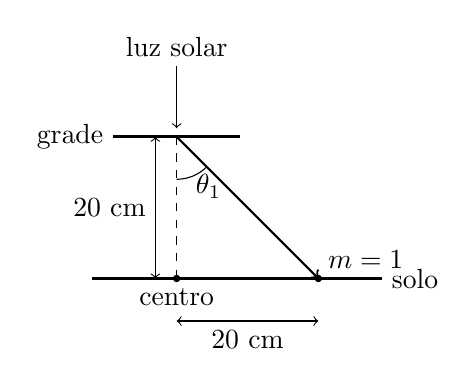
\begin{tikzpicture}[scale=0.9]
  \draw[thick] (-1.2,0) -- (2.9,0);
  \node[right] at (2.9,0) {solo};
  \draw[very thick] (-0.9,2) -- (0.9,2);
  \node[left] at (-0.9,2) {grade};
  \draw[->] (0,3) -- (0,2.12);
  \node[above] at (0,3) {luz solar};
  \draw[dashed] (0,2) -- (0,0);
  \draw[->, thick] (0,2) -- (2,0);
  \draw (0,1.4) arc (-90:-45:0.6);
  \node at (0.45,1.3) {$\theta_1$};
  \fill (0,0) circle (1.5pt);
  \fill (2,0) circle (1.5pt);
  \node[below] at (0,0) {centro};
  \node[above right] at (2,0) {$m=1$};
  \draw[<->] (-0.3,0) -- (-0.3,2);
  \node[left] at (-0.3,1) {$20\ \text{cm}$};
  \draw[<->] (0,-0.6) -- (2,-0.6);
  \node[below] at (1,-0.6) {$20\ \text{cm}$};
\end{tikzpicture}
\end{center}

\textbf{a) Distância entre as ranhuras.}
O máximo de primeira ordem do laranja ($m = 1$) está em $x_1 = 20\ \text{cm} = H$. Logo
\[
\tan\theta_1 = \frac{20}{20} = 1 \quad\Rightarrow\quad \theta_1 = 45^\circ, \qquad \sin\theta_1 = \frac{\sqrt{2}}{2}.
\]
Como $0^\circ < \theta_1 < 90^\circ$, o ângulo é único. A equação da grade usa $\sin\theta$, e não $\tan\theta$. Com $m = 1$:
\begin{align*}
d &= \frac{\lambda_L}{\sin\theta_1} = \frac{600\ \text{nm}}{\sqrt{2}/2} = 600\sqrt{2}\ \text{nm} \\
  &= 6\sqrt{2}\times 10^{-7}\ \text{m} \approx 8{,}5\times 10^{-7}\ \text{m} \quad (\approx 848{,}5\ \text{nm}).
\end{align*}
\textit{Consistência:} $d\sin\theta_1 = 600\sqrt{2}\cdot\frac{\sqrt{2}}{2}\ \text{nm} = \lambda_L$. Além disso, $|m| \le d/\lambda_L = \sqrt{2} \approx 1{,}41$, então o laranja só tem as ordens $m = 0, \pm 1$. Assim, $m = 1$ é a ordem mais alta, e $m = -1$ cai do lado oposto, à mesma distância. Ordem de grandeza: $1/d \approx 1{,}2\times 10^{3}$ ranhuras por milímetro, compatível com grades comerciais.

\textbf{b) Distância do violeta.}
A grade é a mesma, logo $d$ não muda. Para $m = 1$ e $\lambda_V = 400\ \text{nm}$:
\[
\sin\theta_V = \frac{\lambda_V}{d} = \frac{400}{600\sqrt{2}} = \frac{2}{3\sqrt{2}} = \frac{\sqrt{2}}{3} \approx 0{,}471.
\]
Como $\sin\theta_V < 1$ (equivalentemente, $d/\lambda_V = 3\sqrt{2}/2 \approx 2{,}12 > 1$), o máximo de primeira ordem existe. O ângulo é agudo, logo $\cos\theta_V > 0$:
\begin{align*}
\cos\theta_V &= \sqrt{1-\sin^2\theta_V} = \sqrt{1-\frac{2}{9}} = \frac{\sqrt{7}}{3}, \\
\tan\theta_V &= \frac{\sin\theta_V}{\cos\theta_V} = \frac{\sqrt{2}/3}{\sqrt{7}/3} = \frac{\sqrt{2}}{\sqrt{7}} = \frac{\sqrt{14}}{7}.
\end{align*}
Distância no solo:
\[
x_V = H\tan\theta_V = 20\ \text{cm}\cdot\frac{\sqrt{14}}{7} = \frac{20\sqrt{14}}{7}\ \text{cm} \approx 10{,}7\ \text{cm}.
\]

\textbf{Verificações.}
\begin{itemize}
  \item Unidades: $\lambda/d$ é adimensional, pois ambos estão em nm. A grandeza $x = H\tan\theta$ sai em cm, como pedido.
  \item Sentido: o violeta, de menor $\lambda$, tem menor $\sin\theta$ e cai mais perto do centro: $10{,}7\ \text{cm} < 20\ \text{cm}$.
  \item Caso particular: com ângulos pequenos, $x \propto \lambda$ daria $20\cdot 400/600 \approx 13{,}3$ cm. Esse atalho não vale, pois $\theta_1 = 45^\circ$ não é pequeno. O cálculo exato dá $10{,}7$ cm.
  \item Não confundir com o raio: seu comprimento até o solo é $H/\cos\theta_V \approx 22{,}7\ \text{cm}$, mas o pedido é a distância no solo.
\end{itemize}

ANSWER: a) $d = 6\sqrt{2}\times 10^{-7}\ \text{m} \approx 8{,}5\times 10^{-7}\ \text{m}$ (cerca de 848,5 nm); b) $x_V = \dfrac{20\sqrt{14}}{7}\ \text{cm} \approx 10{,}7\ \text{cm}$%
\newpage%
\section*{Questão 10}

\section*{Solução}

\textbf{Hipóteses e referencial.}
\begin{itemize}
\item Referencial $S$ da Terra, tomado como inercial. Terra, Sistema Solar e Sirius estão em repouso mútuo em $S$, de modo que a distância $L = 8{,}6$ anos-luz é medida em $S$.
\item A fronteira do Sistema Solar está em repouso em $S$. Sua dimensão é desprezível frente a $L$, então ela é tomada como o ponto $x = 0$, e $L$ é a distância fronteira--Sirius.
\item Movimento unidimensional: as trajetórias paralelas são tratadas como a mesma reta (direção Terra--Sirius, eixo $x$), sem deslocamento transversal. Logo, as duas naves cruzam a fronteira no mesmo ponto e no mesmo instante, formando um único evento $O = (t_0, 0)$. Fazemos $t_0 = 0$, de modo que $\Delta t = t - t_0 = t$. Os relógios das duas naves são zerados em $O$.
\item As naves têm velocidades constantes (MRU), no sentido $+x$, com $v_1 = 0{,}8c$ e $v_2 = 0{,}6c$. A nave 1 vai à frente.
\item O sinal se propaga no vácuo com velocidade $c$, em todos os referenciais inerciais (postulado de Einstein), e o tempo de emissão é desprezível.
\end{itemize}

Usaremos anos e anos-luz, com $c = 1$ ano-luz/ano, $\beta_1 = 0{,}8$ e $\beta_2 = 0{,}6$.

\textbf{a) Tempo transcorrido na Terra.}

\textit{Passo 1 (chegada da nave 1 a Sirius).} Em $S$, a nave 1 segue $x_1(t) = v_1 t$ (MRU). Ela chega a Sirius ($x = L$) no evento $A$, em
\[
t_A = \frac{L}{v_1} = \frac{8{,}6}{0{,}8} = 10{,}75\ \text{anos}.
\]

\textit{Passo 2 (posição da nave 2 e sentido do sinal).} Em $t_A$, a nave 2 está em
\[
x_2(t_A) = v_2\,t_A = 0{,}6 \cdot 10{,}75 = 6{,}45\ \text{anos-luz}.
\]
Logo, a nave 2 está atrás da nave 1 por $L - x_2(t_A) = 2{,}15$ anos-luz. O sinal é emitido em $A$, na frente da nave 2, e precisa alcançá-la. Portanto, ele viaja no sentido de $x$ decrescente, com velocidade $c$:
\[
x_{\text{sinal}}(t) = L - c\,(t - t_A), \qquad t \geq t_A.
\]

\textit{Passo 3 (encontro).} A recepção ocorre no instante $t_B$ em que a nave 2 e o sinal estão no mesmo ponto, $x_2(t_B) = x_{\text{sinal}}(t_B)$:
\[
v_2\,t_B = L - c\,(t_B - t_A)
\]
\[
(c + v_2)\,t_B = L + c\,t_A = L + \frac{c\,L}{v_1}
\]
\[
\Rightarrow\quad t_B = \frac{L\,(c + v_1)}{v_1\,(c + v_2)}.
\]

Numericamente, com frações exatas,
\[
t_B = \frac{8{,}6 \cdot 1{,}8}{0{,}8 \cdot 1{,}6} = \frac{15{,}48}{1{,}28} = 12{,}09375\ \text{anos} = \frac{387}{32}\ \text{anos}.
\]

Como $t_0 = 0$, o intervalo transcorrido na Terra é $\Delta t = t_B - t_0 = t_B$.

\textit{Verificação aritmética.} A recepção ocorre em $x_B = v_2\,t_B = 7{,}25625$ anos-luz, menor que $L$, como deve ser, pois a nave 2 ainda não chegou a Sirius. O sinal percorre $L - x_B = 1{,}34375$ anos-luz no intervalo $t_B - t_A = 1{,}34375$ anos, ou seja, com velocidade $c$.

\textit{Observação.} $t_B$ é a coordenada de tempo, no referencial $S$ da Terra, do evento de recepção. Se a pergunta fosse o instante em que a Terra observa a recepção, seria preciso somar o atraso da luz $x_B/c = 7{,}25625$ anos, obtendo $19{,}35$ anos. Esse não é o pedido.

\textbf{Resposta a):} $\Delta t = t_B \approx 12{,}1$ anos.

\textbf{b) Tempo transcorrido para os astronautas da nave 2.}

Os eventos $O$ e $B$ estão sobre a linha de universo da nave 2, ou seja, ocorrem no mesmo ponto do referencial dela, e o relógio de bordo foi zerado em $O$. Como a nave 2 está em MRU, seu referencial $S'$ é inercial, e o intervalo medido pelo seu relógio de bordo é o tempo próprio $\Delta\tau$. A dilatação temporal dá
\[
\Delta\tau = \frac{\Delta t}{\gamma_2}, \qquad \gamma_2 = \frac{1}{\sqrt{1 - \beta_2^2}} = \frac{1}{\sqrt{1 - 0{,}36}} = \frac{1}{0{,}8} = 1{,}25,
\]
com $\Delta t = t_B$. Assim,
\[
\Delta\tau = \frac{t_B}{\gamma_2} = 0{,}8 \cdot 12{,}09375 = 9{,}675\ \text{anos} = \frac{387}{40}\ \text{anos}.
\]

\textit{Verificação independente no referencial da nave 2.} Transformamos o evento de emissão $A = (t_A,\ L) = (10{,}75;\ 8{,}6)$ para $S'$, que se move com $u = v_2$ em relação a $S$:
\[
x' = \gamma_2\,(x - v_2\,t), \qquad t' = \gamma_2\left(t - \frac{v_2\,x}{c^2}\right).
\]
\[
t'_A = 1{,}25\,(10{,}75 - 0{,}6 \cdot 8{,}6) = 1{,}25 \cdot 5{,}59 = 6{,}9875\ \text{anos}, \qquad x'_A = 1{,}25\,(8{,}6 - 0{,}6 \cdot 10{,}75) = 1{,}25 \cdot 2{,}15 = 2{,}6875\ \text{anos-luz}.
\]
Em $S'$, a nave 2 está em repouso em $x' = 0$, e o evento $O$ corresponde a $(t' = 0,\ x' = 0)$. O sinal, emitido em $x' = 2{,}6875$ anos-luz e propagando-se em $-x'$ com velocidade $c$ (também em $S'$), chega a $x' = 0$ após $2{,}6875$ anos. Logo, o instante de recepção em $S'$ é
\[
t'_B = 6{,}9875 + 2{,}6875 = 9{,}675\ \text{anos},
\]
que, como $O$ tem $t' = 0$, é o tempo marcado pelo relógio da nave 2. Esse resultado confere com $\Delta\tau$.

\textbf{Resposta b):} $\Delta\tau \approx 9{,}7$ anos.

\textbf{Casos particulares e ordem de grandeza.}
\begin{itemize}
\item $v_1 = v_2$: a fórmula dá $t_B = L/v_1$. As naves permanecem no mesmo ponto, e a recepção ocorre no próprio instante da emissão. Confere.
\item $v_2 \to 0$ (nave 2 parada na fronteira): a fórmula dá $t_B = L/v_1 + L/c$, ou seja, o sinal percorre a distância $L$ de volta a partir de $t_A$. Confere.
\item Dilatação: $\Delta\tau/\Delta t = 0{,}8 = 1/\gamma_2 < 1$. O relógio da nave 2 atrasa em relação ao da Terra, como esperado.
\item Ordem de grandeza: $t_B \sim 10$ anos. Sozinha, a nave 2 levaria $L/v_2 \approx 14{,}3$ anos para chegar a Sirius. A recepção ocorre antes, em $12{,}1$ anos, o que é coerente com o sinal vindo da frente.
\item Unidades: $L/v$ está em anos, e $c\,(t_B - t_A)$ e $x_B$ estão em anos-luz, como esperado.
\end{itemize}

ANSWER: a) 12,1 anos (387/32 anos = 12,09375 anos); b) 9,7 anos (387/40 anos = 9,675 anos)%
\newpage%
\section*{Apêndice: parecer do avaliador}%
\subsection*{Questão 1: nota 8,5 (não aprovada, rodada 3 de 3)}%
\textbf{Resposta da resolução às cegas do avaliador:} a) R\_min = (v$^2$/g) $\cdot$ (cos$\theta$ - $\mu$ sin$\theta$)/(sin$\theta$ + $\mu$ cos$\theta$) = (v$^2$/g) $\cdot$ (1 - $\mu$ tan$\theta$)/(tan$\theta$ + $\mu$). Válido para $\mu$ tan$\theta$ < 1. Se $\mu$ $\geq$ cot$\theta$, não há restrição e R\_min = 0.\newline%
\newline%
b) R\_min = v$^2$/(g tan$\theta$) = (v$^2$/g) cot$\theta$.\newline%
\newline%
c) R\_min = v$^2$/($\mu$ g).\newline%
\newline%
Independentes da massa M. Exemplo com g = 10, v = 10 m/s, $\theta$ = 30$^\circ$, $\mu$ = 0,2: R\_a $\approx$ 11,4 m, R\_b $\approx$ 17,3 m, R\_c = 50 m.\newline%
\newline%
Não há alternativas de múltipla escolha.\par %
Comparação item por item: as três respostas finais coincidem com a referência e foram verificadas independentemente. (a) R\_min = v$^2$/(g$\cdot$tan($\theta$+arctan$\mu$)) = v$^2$(1-$\mu$tan$\theta$)/(g($\mu$+tan$\theta$)) para $\mu$tan$\theta$<1. (b) R\_min = v$^2$/(g$\cdot$tan$\theta$). (c) R\_min = v$^2$/($\mu$g). Caso $\mu$tan$\theta$ $\geq$ 1: ambas as resoluções concluem que não há cota inferior positiva no modelo.\newline%
\newline%
Conferências feitas: (1) A geometria foi lida na figura do PDF renderizada em 300 dpi. A face maior está voltada para o centro do eixo, a geratriz inferior sobe para fora, o trilho apoia{-}se nela, e $\theta$ é o ângulo da geratriz com a horizontal. Ambas as resoluções leram isso corretamente. (2) Um solver independente de vértices e raios do poliedro de equilíbrio (Mg = 1) dá H\_max = tan($\theta$+$\varphi$) para (30$^\circ$, 0,2), (45$^\circ$, 0,3) e (60$^\circ$, 0,5), e ilimitado para (60$^\circ$, 0,6), com $\mu$tan$\theta$ > 1. O ótimo ocorre em N\_I = 0, f\_I = 0, f\_E = -$\mu$N\_E. (3) A família de equilíbrios que o candidato usa para $\mu$tan$\theta$ $\geq$ 1 foi verificada numericamente: H = Mg$\cdot$tan($\varphi$-$\theta$) + s$\cdot$sin2$\theta$/cos($\varphi$-$\theta$) cresce sem limite com s, com N $\geq$ 0 e atrito no limite. (4) A prova de cota inferior ($\Sigma$H $\leq$ tan($\theta$+$\varphi$)$\cdot$$\Sigma$V, com existência por combinação convexa de P* e P0) está correta. (5) Os itens (b) e (c) e as checagens de limite e de unidades estão corretos.\newline%
\newline%
Armadilhas da lista de referência: todas tratadas, exceto a explicitação de por que a roda interna levanta (a normal dela aponta para longe de C). Os problemas restantes são de precisão e redação e não alteram nenhum resultado. A nota é 8,5, e não 9, porque a hipótese (iii) contradiz a análise posterior, a resposta final do caso $\mu$tan$\theta$ $\geq$ 1 não diz R\_min = 0 explicitamente, e o caso N\_w = 0 não foi tratado.%
\begin{itemize}%
\item%
{[}minor{]} A hipótese (iii) diz "O trilho só empurra: N\_w $\geq$ 0", o que contradiz a própria análise do caso $\mu$$\cdot$tan$\theta$ $\geq$ 1, em que a reação total de atrito tem componente vertical negativa (V\_E < 0). Deve{-}se restringir a afirmação à componente normal: a normal só empurra (N\_w $\geq$ 0), mas a reação total pode apontar para baixo quando $\mu$$\cdot$tan$\theta$ $\geq$ 1.%
\item%
{[}minor{]} No passo 2 da cota inferior do item (a), escreve{-}se f\_w = N\_w$\cdot$tan$\beta$\_w, o que não está definido para N\_w = 0. Deve{-}se acrescentar que, nesse caso, R\_w = 0 e a desigualdade $\Sigma$H $\leq$ tan($\theta$+$\varphi$)$\cdot$$\Sigma$V vale trivialmente para essa roda.%
\item%
{[}minor{]} A resposta final do caso $\mu$$\cdot$tan$\theta$ $\geq$ 1 diz apenas "não há cota inferior no modelo". O gabarito deve afirmar explicitamente R\_min = 0 (no modelo, qualquer R > 0 admite contato nas duas rodas), e só depois a ressalva de que a hipótese de corpo rígido deixa de valer. Como está, a conclusão é ambígua.%
\item%
{[}minor{]} Em (b), a afirmação "a roda interna é a que se levanta" não traz a razão física. Deve{-}se explicar que a normal da roda interna aponta para o ponto médio do eixo, isto é, para longe de C, e por isso reduz a força centrípeta. Em (ii), "para o centro do eixo" é ambíguo com o centro de curvatura C e deve ser reescrito.%
\item%
{[}minor{]} A frase "o trilho 'crava' a roda externa (efeito de cunha)" é vaga. O mecanismo exato é a componente vertical do atrito, f$\cdot$sin$\theta$, tornar{-}se negativa e vencer a normal quando f < -N$\cdot$cot$\theta$, o que só é possível se $\mu$ $\geq$ cot$\theta$. Vale escrever essa condição, pois ela é a origem do caso de exceção.%
\end{itemize}%
\subsection*{Questão 2: nota 8,0 (não aprovada, rodada 3 de 3)}%
\textbf{Resposta da resolução às cegas do avaliador:} a) Forças normais, perpendiculares ao plano:\newline%
N\_A = g cos$\theta$ $\cdot$ {[} M/2 + (m(L - a - d) + m\_c(b - d)) / (L - 2d) {]}\newline%
N\_B = g cos$\theta$ $\cdot$ {[} M/2 + (m(a - d) + m\_c(L - b - d)) / (L - 2d) {]}\newline%
Verificação: N\_A + N\_B = (M + m + m\_c) g cos$\theta$.\newline%
\newline%
b) Atrito, paralelo ao plano, no sentido de subida:\newline%
{-} Soma determinada: f\_A + f\_B = (M + m + m\_c) g sin$\theta$.\newline%
{-} Individualmente, a estática não determina a divisão. Com a hipótese de deslizamento iminente e mesmo coeficiente nos dois apoios ($\mu$ = tan$\theta$), resulta f\_A = tan$\theta$$\cdot$N\_A = g sin$\theta$ $\cdot$ {[} M/2 + (m(L - a - d) + m\_c(b - d))/(L - 2d) {]} e f\_B = tan$\theta$$\cdot$N\_B = g sin$\theta$ $\cdot$ {[} M/2 + (m(a - d) + m\_c(L - b - d))/(L - 2d) {]}.\newline%
\newline%
Válido para 0 < d < L/2, com N\_A, N\_B $\geq$ 0 e $\mu$\_e $\geq$ tan$\theta$. Não há alternativa de múltipla escolha.\par %
Resposta final correta e idêntica à de referência. Conferi com python: N\_A = g cos$\theta$/(L-2d)$\cdot${[}M(L/2-d)+m(L-a-d)+m\_c(b-d){]} e N\_B análogo satisfazem as três equações independentes (força normal, força paralela e momento) com resíduo \textasciitilde{}1e-14. Os valores do exemplo (N\_A$\approx$57,9 N, N\_B$\approx$54,7 N, f\_A$\approx$33,4 N, f\_B$\approx$31,6 N, tan30$^\circ$$\approx$0,577) e a variação de 0,41 N para $\delta$ = 1 cm também conferem. Todos os itens de a) e b) estão respondidos. Em b), a estática fixa só f\_A + f\_B = (M+m+m\_c) g sin$\theta$. A repartição individual é declarada como hipótese de mobilização uniforme (f\_i/N\_i = tan$\theta$), e isso fica explícito na resposta final. Armadilhas tratadas: cos vs sin, posições a/b/d, centro de massa em L/2, braços de momento, sentido do atrito, indeterminação, validade N $\geq$ 0, caso L = 2d e casos{-}limite. Faltou: a justificativa de que o atrito não gera momento está imprecisa; a afirmação de que a altura $\delta$ é 'obrigatória' é superestimada (a resposta é independente de $\delta$ se o atrito atuar na altura da barra); há um non sequitur na positividade das frações; e há omissões de rigor (componente lateral do atrito, bounds de a e b). Não há erro que mude a resposta. A nota fica abaixo de 9 por esses problemas de justificativa, não por erro de conta.%
\begin{itemize}%
\item%
{[}minor{]} A Hipótese 1 afirma que a idealização de contatos no plano ($\delta$ = 0) é 'obrigatória' e que a altura $\delta$ alteraria N\_A e N\_B em $\pm$$\delta$ g sin$\theta$ (M+m+m\_c)/(L-2d). Isso só vale se o atrito atuar na superfície do plano (h = 0) enquanto os pesos estão a altura $\delta$. Refiz a conta: se o atrito atuar na altura da barra (configuração da figura, em que a barra repousa sobre os suportes), o termo em $\delta$ se cancela exatamente, porque a soma dos momentos das forças tangenciais é $\delta$$\cdot$($\Sigma$ forças tangenciais) = 0, e as fórmulas de N\_A e N\_B continuam valendo para qualquer $\delta$. A afirmação de necessidade está errada como enunciada. O correto seria dizer que o resultado assume contatos sobre o plano e que, nessa hipótese, $\delta$ precisaria ser conhecido. A quantificação de 0,4 N está correta apenas para esse modelo. A resposta final não muda, mas a justificativa da hipótese está mal formulada. Deveria ser corrigida para explicitar onde atuam as forças tangenciais.%
\item%
{[}minor{]} Em Item b, a frase 'Ambas as frações são positivas, pois o atrito atua para cima do plano' é um non sequitur. A positividade de f\_i = N\_i tan$\theta$ depende de N\_i $\geq$ 0, que é uma condição de validade, e não do sentido do atrito, que é uma convenção de sinal. Deveria ser: 'f\_i $\geq$ 0 porque N\_i $\geq$ 0 (condição de validade)'.%
\item%
{[}minor{]} A justificativa do momento nulo de F\_s ê\_s ('atua ao longo da própria linha da barra, que contém o eixo') é imprecisa. O eixo é perpendicular a $\Pi$, e a linha da barra está contida em $\Pi$, então ela não contém o eixo. O motivo correto é que a força é colinear com o braço (ambos ao longo de ê\_s, com altura nula). Além disso, 'plano $\Pi$ da barra' nunca é definido e pode ser lido como o plano inclinado. Deveria definir{-}se $\Pi$ como o plano (ê\_s, ê\_n).%
\item%
{[}minor{]} A componente lateral do atrito (fora do plano de ê\_s e ê\_n) é assumida nula sem justificativa. A hipótese 'todas as forças atuam nessa linha' também não é exata, pois as normais são perpendiculares à linha. A estática implica f\_Ay = f\_By = 0: f\_Ay + f\_By = 0 e d$\cdot$f\_Ay + (L-d)$\cdot$f\_By = 0, com determinante L-2d $\neq$ 0. Esse argumento deveria aparecer.%
\item%
{[}minor{]} A justificativa para f\_A = f\_B ('contatos idênticos e elásticos com a barra transladando sem girar') é solta. Além disso, a repartição por mobilização uniforme (f\_i/N\_i constante) é uma escolha de modelo. O texto a declara, mas o parágrafo de validade poderia deixar mais claro que a única parte determinada pela estática é a soma.%
\item%
{[}minor{]} A resolução é longa e inclui itens não exigidos (exemplo numérico com valores arredondados sem contas intermediárias, parágrafo de unidades, várias conferências). Isso é um risco real de caber mal no espaço de resposta do caderno de soluções. Se o exemplo numérico for mantido, a instrução 8 pede que as expressões numéricas sejam resolvidas integralmente.%
\item%
{[}minor{]} A seção de validade não cobre todos os casos: não exige 0 $\leq$ a, b $\leq$ L nem d > 0, e não dá exemplos físicos de quando N\_A ou N\_B se tornam negativas (m perto de A, m\_c além de B).%
\end{itemize}%
\subsection*{Questão 3: nota 9,0 (aprovada, rodada 3 de 3)}%
\textbf{Resposta da resolução às cegas do avaliador:} (a) Componente radial da reação do pivô, ao longo da haste (orientada da extremidade inferior para o pivô):\newline%
    N\_r = M {[} g cos $\theta$ + $\omega$$^2$(L/2 - a) {]} = (M/2){[} 2g cos $\theta$ + $\omega$$^2$(L - 2a) {]}\newline%
  Independe de $\alpha$ e do momento de inércia. Se a convenção for "positiva para fora do pivô", o sinal troca.\newline%
\newline%
(b) Ângulo que anula a componente radial:\newline%
    cos $\theta$ = $\omega$$^2$(2a - L)/(2g)  $\Rightarrow$  $\theta$ = arccos{[} $\omega$$^2$(2a - L)/(2g) {]}\newline%
  Existe apenas se |$\omega$$^2$(L - 2a)| $\leq$ 2g. A massa M não aparece na resposta, pois cancela.\newline%
  Para a < L/2, $\theta$ $\in$ (90$^\circ$, 180$^\circ${]}; para a > L/2, $\theta$ $\in$ {[}0$^\circ$, 90$^\circ$); para a = L/2, $\theta$ = 90$^\circ$.\newline%
\newline%
Observação: a questão está na página 4 do PDF, que tem 12 páginas (o enunciado indicava 4). O conteúdo de Q3 foi conferido nessa página.\par %
Resposta final correta e igual à de referência nos dois itens, com a mesma convenção de sinal: N\_r > 0 quando a reação aponta no sentido do trecho inferior para o pivô (-ê\_r). (a) N\_r = M{[}g cos$\theta$ + $\omega$$^2$(L/2 - a){]}; (b) $\theta$ = arccos{[}$\omega$$^2$(2a-L)/(2g){]}, com existência $\omega$$^2$|L-2a| $\leq$ 2g, M cancelando. Verifiquei com Python em 10 000 casos aleatórios (erro relativo \textasciitilde{}1e{-}14) que N\_r, F\_t = Mg L$^2$ sin$\theta$/{[}L$^2$+3(L-2a)$^2${]} e $\alpha$ = -6g(L-2a)sin$\theta$/{[}L$^2$+3(L-2a)$^2${]} estão corretos. O exemplo numérico do candidato (L=1, a=0,25, $\omega$=2, g=10 $\to$ cos$\theta$ = -0,1, $\theta$ $\approx$ 95,7$^\circ$, N\_r = 0) confere. A leitura de a como trecho superior, d = L/2 - a, o uso de cos$\theta$, a projeção de $\omega$$^2$ e a checagem de a = L/2 e de $\omega$ = 0 estão corretos. Todas as armadilhas da lista foram tratadas: convenção de sinal declarada, $\theta$ > 90$^\circ$ válido, M cancela, condição de existência, N\_r diferente da reação total, I\_O por Steiner. A justificativa é completa e rigorosa. Os problemas restantes são de redação e de rigor pontual (afirmação de checagem não demonstrada, non sequitur sobre o intervalo de $\theta$, sinal do termo centrípeto não explicitado), sem impacto no conteúdo. Com esses ajustes, a resolução poderia sair como gabarito comentado."\}{]}%
\begin{itemize}%
\item%
{[}minor{]} A 'Conferência independente' afirma que derivar numericamente a trajetória de G e aplicar o passo 1 dá os mesmos N\_r e F\_t, mas não mostra nenhum valor nem procedimento. A afirmação é verdadeira (verifiquei), mas não está demonstrada no texto. Deve{-}se mostrar os números da checagem ou remover a frase.%
\item%
{[}minor{]} A hipótese '$\theta$ medido a partir da vertical descendente, no sentido de +x, como na figura, logo $\theta$$\in${[}0,$\pi${]}' é um non sequitur: medir no sentido de +x dá intervalo {[}0,2$\pi$). A restrição a {[}0,$\pi${]} corresponde a supor a parte inferior do lado direito, e não à figura. Mais adiante, 'a convenção da figura fixa $\theta$$\in${[}0,$\pi${]}' superestima o que a figura mostra. Deveria ser dito que $\theta$ é o ângulo não orientado entre a haste (parte inferior, à direita) e a vertical descendente, que a configuração espelhada corresponde a -$\theta$, e que a resposta completa é $\theta$ = $\pm$arccos{[}$\omega$$^2$(2a-L)/(2g){]}. O '$\pm$' não aparece na resposta final.%
\item%
{[}minor{]} No Passo 3, 'O termo M$\omega$$^2$d é a força centrípeta de G' omite o sinal. A força centrípeta é -M$\omega$$^2$d ê\_r, e a expressão F$\cdot$ê\_r = -M$\omega$$^2$d - Mg cos$\theta$ depende desse sinal. O sentido é corrigido na frase seguinte, mas o texto deveria escrever o termo com o sinal explícito para não gerar ambiguidade.%
\end{itemize}%
\subsection*{Questão 4: nota 8,5 (não aprovada, rodada 3 de 3)}%
\textbf{Resposta da resolução às cegas do avaliador:} a) y2 = 2b ou y2 = -4b. Ambas são válidas, porque o centro de massa dos fragmentos, (4a/5, (b + y2)/5), cai na elipse nos dois casos.\newline%
\newline%
b) Menor energia potencial (U = 0 no infinito, estrela em um foco, termo mútuo desprezado por M ? m):\newline%
U\_min = -(GMm/5) {[} 16/$\surd$(25a$^2$ - 15b$^2$ - 24a$\cdot$c) + 1/$\surd$(2a$^2$ + 3b$^2$ - 2a$\cdot$c) {]}, com c = $\surd$(a$^2$ - b$^2$).\newline%
Obtida com a estrela no foco (+c, 0) e y2 = 2b. Para a = 5, b = 3 (c = 4), U\_min $\approx$ -1,045 GMm.\newline%
Se o termo mútuo entre fragmentos for incluído, soma{-}se -16Gm$^2$/(25$\surd$(a$^2$ + 49b$^2$)), uma correção de ordem m/M.\par %
Resposta final correta e igual à da referência. (a) y2 = 2b ou y2 = -4b, pois o CM (4a/5, (b+y2)/5) deve estar sobre a elipse, e as duas raízes são válidas. (b) U\_min = -(GMm/5){[}16/$\surd$(25a$^2$-15b$^2$-24ac) + 1/$\surd$(2a$^2$+3b$^2$-2ac){]}, com a estrela no foco (+c, 0) e y2 = 2b. A correção mútua é -16Gm$^2$/(25$\surd$(a$^2$+49b$^2$)). Conferi o enunciado no PDF e as contas: as identidades algébricas, os valores da tabela (-5,224; -5,143; -0,606; -0,580), a razão 0,028 m/M e a escolha de foco e de y2 por brute force em sete pares (a,b). Todas as armadilhas da referência foram tratadas: P2 não precisa estar na elipse, pesos 4/5 e 1/5, a raiz -4b, a estrela em foco e não na origem, a escolha do foco e de y2 com justificativa, U = 0 no infinito, o termo mútuo justificado por ordem m/M, e a verificação na elipse. O problema é de forma, não de física: premissa do CM mal descrita, total do item (b) não escrito como uma expressão, afirmação não auditável e excesso de material para o caderno. A nota fica em 8,5, abaixo de 9, porque falta limpeza na apresentação para um gabarito comentado.%
\begin{itemize}%
\item%
{[}minor{]} A premissa do centro de massa está mal delimitada. O texto diz que ela é 'adotada pelo enunciado', mas o enunciado não a afirma, e diz que é 'exata no instante da cisão'. O instante dado tem P1 $\neq$ P2, então não é o instante da cisão. A resposta de (a) depende dessa hipótese. O correto seria declará{-}la como hipótese explícita (o CM dos fragmentos permanece sobre a elipse no instante considerado) e mencionar a aproximação uma única vez. A formulação 'o erro real é grande' enfraquece a resposta sem necessidade.%
\item%
{[}minor{]} No item (b), a linha de resposta traz só a energia estelar e a correção mútua aparece separada. O total U\_min,total = U\_* + U\_mut nunca é escrito como uma expressão única. O correto seria escrever U\_min,total = -(GMm/5){[}\ldots{}{]} - 16Gm$^2$/(25$\surd$(a$^2$+49b$^2$)) e depois dizer que, com M ? m, o termo mútuo é desprezado na resposta principal.%
\item%
{[}minor{]} A frase 'repeti a comparação por força bruta em seis pares (a,b)' não traz saída, tabela nem critério de amostragem, então não é auditável. Deveria mostrar o resultado ou ser removida. Refiz a verificação em sete pares (a,b) com brute force e a conclusão se mantém: mínimo em (+c, 2b), com e sem o termo mútuo, e a forma fechada bate com o brute force até 1e{-}6.%
\item%
{[}minor{]} O argumento de escolha do foco (Passo 3) usa desigualdades estritas, que exigem c > 0. No caso degenerado b = a (c = 0) os focos coincidem e a escolha é irrelevante. Isso deveria ser dito, porque o caso aparece depois nas verificações.%
\item%
{[}minor{]} A resolução tem material demais para o caderno de soluções, onde a prova só aceita respostas nos espaços delimitados. A tabela de quatro combinações, o sweep de pares, a discussão do limite b $\to$ 0 e a verificação de unidades não são exigidos. Uma versão publicável teria: hipótese do CM, pesos 4/5 e 1/5, equação em y2 com as duas raízes, comparação das distâncias para escolher foco e y2, U\_min com a justificativa do termo mútuo. Esse conjunto cabe numa página.%
\end{itemize}%
\subsection*{Questão 5: nota 7,5 (não aprovada, rodada 3 de 3)}%
\textbf{Resposta da resolução às cegas do avaliador:} a) Trabalho total por ciclo: W = (M1 - M2)$\cdot$g$\cdot$$\alpha$$\cdot$L$\cdot$$\Delta$T, com $\Delta$T = 70 K. Logo W = 70$\cdot$g$\cdot$$\alpha$$\cdot$L$\cdot$(M1 - M2) = 700$\cdot$$\alpha$$\cdot$L$\cdot$(M1 - M2) (J, com g = 10 m/s$^2$). É positivo se M1 > M2. Não é só o trabalho do aquecimento.\newline%
\newline%
b) Eficiência: $\eta$ = W/Q\_H = (M1 - M2)$\cdot$g$\cdot$$\alpha$$\cdot$L / ($\rho$\_H2O$\cdot$V$\cdot$c\_H2O + 3mR/M\_Cu + M1$\cdot$g$\cdot$$\alpha$$\cdot$L). Com g = 10: $\eta$ = 10$\cdot$$\alpha$$\cdot$L$\cdot$(M1 - M2) / ($\rho$\_H2O$\cdot$V$\cdot$c\_H2O + 3mR/M\_Cu + 10$\cdot$$\alpha$$\cdot$L$\cdot$M1). É adimensional e muito menor que o limite de Carnot ($\approx$ 0,19). Não há alternativa de múltipla escolha.\par %
A resposta final do candidato está correta e coincide com a referência. a) W = (M1-M2)$\cdot$g$\cdot$$\alpha$$\cdot$L$\cdot$$\Delta$T = 700$\cdot$$\alpha$$\cdot$L$\cdot$(M1-M2) J, positivo se M1 > M2. b) $\eta$ = (M1-M2)$\cdot$g$\cdot$$\alpha$$\cdot$L / ($\rho$\_H2O$\cdot$V$\cdot$c\_H2O + 3Rm/M\_Cu + M1$\cdot$g$\cdot$$\alpha$$\cdot$L). Conferi: $\Delta$T = 70 K; Q = $\Delta$U + W em cada trecho com carga; Q\_H - Q\_F = W; o exemplo numérico (W $\approx$ 0,0595 J, Q\_H $\approx$ 2,96$\times$10$^{6}$ J, $\eta$ $\approx$ 2,0$\times$10$^{-}$$^{8}$) e a razão do termo M1g$\alpha$L no denominador ($\approx$4$\times$10$^{-}$$^{8}$) estão corretos; a razão do peso próprio ($\approx$2,2$\times$10$^{-}$$^{7}$$\cdot$L) e a cota de Clausius 1 - 293/363 $\approx$ 0,193 também. Todas as armadilhas da referência foram tratadas, exceto a independência da área, que não foi citada. A resolução principal tem nível de gabarito, mas a parte não pedida tem problemas reais: uma cota de 2ª lei derivada de uma premissa que a própria solução declara falsa; a atribuição errada da inconsistência a Dulong{-}Petit (os termos de C se cancelam); e uma estimativa de erro da linearização que vale para o comprimento final, não para $\Delta$L ($\approx$6$\times$10$^{-}$$^{4}$, não 10$^{-}$$^{6}$). A tese de que o modelo não é termodinamicamente consistente é defensável, mas está mal delimitada. Nota 7,5: não chega a 9 por causa dessas afirmações falsas ou contraditórias, que um gabarito não poderia publicar.%
\begin{itemize}%
\item%
{[}major{]} Na observação sobre a segunda lei, a cota $\eta$ $\leq$ 1 - 293/T\_F é derivada de $\Delta$S\_univ = Q\_F/T\_0 - Q\_H/T\_F $\geq$ 0. Isso pressupõe $\Delta$S\_viga = 0 no ciclo, exatamente o que a própria observação declara falso ('a força não é função de estado'). É uma conclusão apresentada como válida que contradiz a premissa do próprio texto. Deveria ser removida, ou explicitamente condicionada a um sistema consistente, mantendo apenas a cota de Clausius ($\eta$ $\leq$ 1 - 293/363) que vale para corpo consistente.%
\item%
{[}minor{]} A hipótese 7 afirma que a lei de Dulong{-}Petit é 'a que torna o modelo inconsistente'. Isso é falso: os termos de capacidade térmica C se cancelam em ?dS (C$\cdot$ln(363/293) - C$\cdot$ln(363/293) = 0), como a própria conta da observação mostra. A inconsistência vem da força da carga (f dL = Mg$\cdot$$\alpha$L dT) tratada como se fosse função de estado, junto com as trocas M1?M2 supostas sem variação de entropia. Deveria corrigir a atribuição e apontar a hipótese realmente conflitante.%
\item%
{[}minor{]} Estimativa de erro da linearização mal calculada. ($\alpha$$\Delta$T)$^2$/2 $\approx$ 7$\times$10$^{-}$$^{7}$ é o erro relativo do comprimento final L/L0 (verificado). O erro relativo em $\Delta$L, que é o que entra em W e $\eta$, é $\approx$ $\alpha$$\Delta$T/2 $\approx$ 6$\times$10$^{-}$$^{4}$ (verificado), cerca de 10$^3$ vezes maior. A conclusão de usar $\Delta$L = $\alpha$L$\Delta$T permanece válida pela convenção do enunciado, mas a justificativa numérica está errada. Deveria corrigir o número, definir L como comprimento inicial L0 e nomear a lei exponencial corretamente (L = L0$\cdot$e\^{}\{$\alpha$$\Delta$T\} para dL = $\alpha$L dT).%
\item%
{[}minor{]} A inconsistência do modelo é afirmada sem ser delimitada. A solução diz que o modelo não é consistente e que as cotas de 2ª lei não se aplicam 'sem ressalva', mas não discute se a premissa de $\Delta$S = 0 nas trocas de carga (hipótese 6, sem calor e sem deslocamento) é a que falha, nem se as respostas pedidas em a) e b) continuam sendo as pretendidas dentro do modelo do enunciado. Deveria apontar a hipótese conflitante em uma frase e dizer que a e b são as respostas no modelo idealizado.%
\item%
{[}minor{]} Hipóteses desprezadas sem justificativa adequada. (i) Pressão atmosférica: não altera W (o trabalho atmosférico se anula no ciclo), mas altera Q\_H; a área não é dada ($\rho$\_Cu não está no enunciado), e no próprio exemplo P\_atm$\cdot$A $\approx$ 11 N contra M1$\cdot$g = 100 N, embora o efeito em $\eta$ seja numericamente desprezível. (ii) Empuxo da viga, já que a viga está no banho. (iii) Volume da viga desprezado frente a V ($\approx$1\% no exemplo). (iv) $\rho$\_H2O constante, quando a densidade varia $\approx$3\% entre 20 e 90 $^\circ$C. Deveria justificar em uma linha cada ou declarar que são aproximações sem efeito na forma simbólica pedida.%
\item%
{[}minor{]} A armadilha 'o trabalho não depende da área da seção' (W = F$\cdot$$\Delta$L, P = F/A, V = A$\cdot$?) não é mencionada. A solução usa W = $\int$N dy, o que é correto, mas deveria afirmar explicitamente que A não entra no resultado.%
\item%
{[}minor{]} Excesso de material não pedido em espaço de caderno limitado: observação termodinâmica longa, exemplo numérico com dados externos, refinamentos e cálculos de ordem de grandeza. A resposta final fica no fim do texto. Um gabarito comentado deveria trazer só o cálculo principal, a verificação da 1ª lei (Q\_H - Q\_F = W) e as duas respostas, com as ressalvas em uma frase cada.%
\end{itemize}%
\subsection*{Questão 6: nota 8,5 (não aprovada, rodada 3 de 3)}%
\textbf{Resposta da resolução às cegas do avaliador:} a) L = f1 + f2 = 80 + 5,0 = 85 cm (0,85 m), no ajuste normal (imagem final no infinito).\newline%
\newline%
b) G = f1/f2 = 80/5,0 = 16 em módulo (G = -16 com a convenção de sinal, que indica inversão). A imagem final é invertida (de cabeça para baixo, rotação de 180$^\circ$), como em toda luneta kepleriana com duas lentes convergentes.\newline%
\newline%
c) Objetiva: imagem intermediária virtual e direita, a 80 cm à frente da objetiva (lado do objeto), com tamanho 2 vezes maior, pois o objeto está entre o foco e a objetiva.\newline%
Ocular: imagem final real e invertida em relação ao objeto, a 165/32 $\approx$ 5,16 cm atrás da ocular ($\approx$ 90,2 cm da objetiva), com aumento linear total A = -1/16.\newline%
A imagem final é MENOR que o objeto, 16 vezes menor.\par %
Parecer sobre a Questão 6 (luneta astronômica, ITA 2026, Física). Enunciado conferido na página 7 do PDF: f1 = +80 cm, f2 = +5,0 cm, objeto a 40 cm da objetiva.\newline%
\newline%
Comparação item por item:\newline%
{-} (a) Candidato: L = 85 cm (0,85 m). Referência: 85 cm. Concordam. Correto, pois no ajuste normal o foco imagem da objetiva coincide com o foco objeto da ocular.\newline%
{-} (b) Candidato: G = 16 em módulo (-16 na convenção algébrica), imagem invertida (girada de 180$^\circ$), virtual e no infinito. Referência: o mesmo. Concordam. Correto. A inversão f2/f1 = 1/16 foi descartada na derivação.\newline%
{-} (c) Candidato: objetiva p1' = -80 cm, m1 = +2 (virtual, direita, 80 cm à frente da objetiva). Ocular: p2 = +165 cm (objeto real), p2' = 165/32 $\approx$ 5,16 cm (real, atrás da ocular, $\approx$ 90,2 cm da objetiva), m2 = -1/32. Total m = -1/16, imagem menor (16 vezes). Referência: o mesmo. Concordam. Verifiquei com frações exatas em python3. A alternativa com p2 = -165 cm daria 165/34 cm, que ambos rejeitaram corretamente.\newline%
\newline%
Não há divergência de resposta final. A resposta está correta e é rigorosa: todas as contas estão integrais e as convenções de sinal estão declaradas. Os problemas são de justificativa e de redação. Há uma afirmação falsa no contraste com a galileana (major) e três lacunas menores. Por isso a nota fica em 8,5 e não chega a 9, que exigiria gabarito publicável sem correções.\newline%
\newline%
Armadilhas da referência: todas tratadas, exceto a menção explícita a f1 - f2 = 75 cm e a f2/f1 = 1/16, que ficaram implícitas."%
\begin{itemize}%
\item%
{[}major{]} No trecho de contraste com a luneta galileana, a frase 'Aplicar essas fórmulas à luneta kepleriana daria imagem direita' é falsa. Com f2 > 0, G = -f1/f2 = -16, e pela própria convenção do texto (sinal negativo = inversão) isso indica imagem invertida, não direita. Além disso, L = f1 - |f2| daria 75 cm, que está errado. Deve ser reescrita: dizer que a leitura galileana (G > 0 $\Rightarrow$ direita; L = f1 - |f2| = 75 cm) não vale para a kepleriana, ou remover a frase.%
\item%
{[}minor{]} A hipótese de ajuste normal (imagem final no infinito, logo L = f1 + f2) é afirmada nas hipóteses, mas não é ligada explicitamente à frase do enunciado 'imagens dos objetos celestes observadas são formadas a longas distâncias do observador'. Essa frase é a justificativa do ajuste e deveria ser citada, pois é ela que fixa a escolha de L.%
\item%
{[}minor{]} Armadilhas não nomeadas: L = f1 - f2 = 75 cm e G = f2/f1 = 1/16 não são mencionados. O candidato evita ambos pela derivação $\beta$/$\alpha$ e pelo diagrama de raios, mas um gabarito comentado deveria alertar explicitamente sobre os dois erros comuns.%
\item%
{[}minor{]} Em (b), 'A ocular funciona como lupa sobre essa imagem' é impreciso. Como a imagem intermediária está exatamente em F2, a ocular colima os raios (saem paralelos) e não forma imagem ampliada no regime de lupa, que exige objeto entre o foco e a lente. Deveria dizer que a ocular colima os raios.%
\end{itemize}%
\subsection*{Questão 7: nota 8,5 (não aprovada, rodada 3 de 3)}%
\textbf{Resposta da resolução às cegas do avaliador:} a) I\_f = x\^{}(N+1) $\cdot$ I0 $\cdot$ cos\^{}(2N)($\varphi$/N)\newline%
\newline%
b) r = sqrt( P / ($\pi$ $\cdot$ x\^{}(N+1) $\cdot$ I0 $\cdot$ cos\^{}(2N)($\varphi$/N)) ) = (1/cos\^{}N($\varphi$/N)) $\cdot$ sqrt( P / ($\pi$ $\cdot$ x\^{}(N+1) $\cdot$ I0) )\newline%
\newline%
Não há alternativas de múltipla escolha nesta questão.\par %
Nota 8,5/10. A resposta final do candidato coincide com a referência nos dois itens: a) I = x\^{}\{N+1\}$\cdot$I0$\cdot$cos\^{}\{2N\}($\varphi$/N), independente de P; b) r = $\surd$(P/($\pi$$\cdot$x\^{}\{N+1\}$\cdot$I0$\cdot$cos\^{}\{2N\}($\varphi$/N))) = |cos($\varphi$/N)|\^{}\{{-}N\}$\cdot$$\surd$(P/($\pi$$\cdot$x\^{}\{N+1\}$\cdot$I0)). Confirmei no PDF (p. 8) que o enunciado é o da transcrição, incluindo "após a passagem por cada polarizador" e "fração x daquela que seria obtida em um caso ideal". Com python confirmei que a recorrência I\_k = x$\cdot$cos$^2$$\beta$$\cdot$I\_\{k{-}1\} coincide com a forma fechada (diferença $\leq$ 1,5$\cdot$10$^{-}$$^{1}$$^2$), que o exemplo N=2 dá 182,25 (composta) e 225 (alternativa), que I$\cdot$$\pi$r$^2$ = 1 W para P = 1 W, que N=10 dá 283,9 e N=100 dá 0,0237 W/m$^2$, e que o exemplo N=3 dá 45,17 W/m$^2$ e r $\approx$ 4,2 mm. Todos os números do candidato conferem. Quanto às armadilhas: $\varphi$ = N$\beta$ com N passos, expoentes 2N e x\^{}\{N+1\}, substituição $\beta$ $\to$ $\varphi$/N, distinção entre intensidade e potência (P = I$\cdot$$\pi$r$^2$), P fora do item a, analisador tratado como medidor sem perda, uniformidade do perfil, limite N$\to$$\infty$ com x<1 (I$\to$0) e o caso cos($\varphi$/N)=0 foram tratados. Lacunas: um erro de expoente numa checagem (cos$^2$ em vez de cos$^{4}$), a checagem de N=1 sem x, justificativa textual curta da leitura composta e excesso de extensão para o espaço da prova."%
\begin{itemize}%
\item%
{[}minor{]} Na checagem 'Usar $\varphi$ no lugar de $\beta$ daria I0 cos$^2$($\pi$/2)=0', o expoente está errado: para N=2 a fórmula com $\varphi$ no lugar de $\beta$ seria cos\^{}\{2N\}($\varphi$) = cos$^{4}$($\pi$/2). O valor resultante (zero) não muda, mas a expressão escrita não corresponde à fórmula do próprio texto. Deveria ser corrigida para cos$^{4}$($\pi$/2).%
\item%
{[}minor{]} A checagem de N=1 exigida pela referência (I = x$^2$$\cdot$I0$\cdot$cos$^2$$\varphi$) não aparece explicitamente. Só se verificou N=1 com x=1 (Malus clássica). A fórmula geral reduz a esse caso, mas a verificação com a perda x, que testaria o expoente de x, deveria ser mostrada.%
\item%
{[}minor{]} A escolha da leitura composta de x (um fator de x por polarizador, multiplicativo) está bem argumentada e a leitura alternativa é identificada e quantificada (225 vs 182,25 W/m$^2$ no exemplo). Porém a justificação textual é curta: 'caso ideal' é ambíguo, e o texto só diz que x se aplica 'após a passagem por cada polarizador'. A resolução deveria explicitar que o 'caso ideal' do polarizador k é a ação ideal sobre a luz que ele realmente recebe, em vez de apoiar{-}se sobretudo em argumento físico. Não é erro, mas é o ponto de maior risco de interpretação da questão.%
\item%
{[}minor{]} No exemplo numérico (0,9$^{4}$$\cdot$cos$^{6}$(20$^\circ$)$\cdot$100 $\approx$ 45,17), o valor de cos(20$^\circ$) não é apresentado, e as expressões são arredondadas. As Instruções Gerais (item 8) exigem resolver as expressões numéricas integralmente. A checagem não altera a resposta simbólica, mas a expressão deveria ser completada ou apresentada como verificação aproximada.%
\item%
{[}minor{]} Extensão e formato: a resolução é longa (seção de leitura alternativa, sete verificações, caso cos=0 detalhado). As instruções exigem que a resolução caiba nos espaços delimitados do caderno de soluções (item 7). Um gabarito comentado deveria ser condensado, mantendo a recorrência, a solução da recorrência, a verificação dos expoentes e as checagens essenciais (N=1 com x, limite com x<1).%
\end{itemize}%
\subsection*{Questão 8: nota 8,0 (não aprovada, rodada 3 de 3)}%
\textbf{Resposta da resolução às cegas do avaliador:} a) P\_min = 35 W (energia mínima do carregador 42 kJ = 36 kJ da bateria + 6 kJ de aquecimento do aparelho, em 1200 s). Não há alternativas de múltipla escolha.\newline%
\newline%
b) $\Delta$t\_max = 2,8$\cdot$M = 22,4$\pi$$^2$$\times$10$^{-}$$^{7}$ s $\approx$ 2,2$\times$10$^{-}$$^{5}$ s (cerca de 22 µs), com M = $\mu$0$\cdot$N$^2$$\cdot$A/? = 8$\pi$$^2$$\times$10$^{-}$$^{7}$ H $\approx$ 7,9 µH e N = 40 espiras.\par %
Resposta final correta nos dois itens e igual à referência. (a) P\_min = 35 W: 36 kJ da bateria + 6 kJ de aquecimento = 42 kJ em 1200 s, com a energia de aquecimento incluída. (b) $\Delta$t\_max = 14L/V = 2,24$\pi$$^2$$\times$10$^{-}$$^{6}$ s $\approx$ 2,2$\times$10$^{-}$$^{5}$ s, com L = $\mu$0$\cdot$n$^2$$\cdot$?$\cdot$A = 8$\pi$$^2$$\times$10$^{-}$$^{7}$ H e M = L por acoplamento perfeito. Refiz todas as contas em python3 e elas conferem, inclusive a cota energética 42 kJ/($\frac12$LI$^2$) e o número de ciclos $\approx$ 5,4$\times$10$^{7}$. Pontos fortes: o candidato detectou corretamente o erro de impressão em $\mu$0 (a página 2 do PDF imprime N$\cdot$A$^{-}$$^{1}$; a unidade correta é N/A$^2$) e usou o valor certo; declarou hipóteses; tratou todas as armadilhas listadas (calor, conversões de Ah, g e J/(g$^\circ$C), N = 40 espiras, área em m$^2$, k = 1, M no lugar de L/2, sinal da cota com 42 kJ, $\Delta$t versus 20 min, potência média versus instantânea); provou |M| $\leq$ L. Fraquezas: a justificativa do máximo depende de uma hipótese energética não derivada, em vez de usar a unicidade imposta pela f.e.m. constante; a reinicialização da corrente não é tratada; há digressões (Wheeler, frequência) que introduzem números extras e uma afirmação imprecisa. Para publicar como gabarito comentado, faltam essas correções de rigor e enxugamento. Nota 8."%
\begin{itemize}%
\item%
{[}major{]} A justificativa do 'máximo' em (b) depende da hipótese H3 (energia transferida por ciclo $\leq$ $\frac12$LI$_{0}$$^2$), declarada sem derivação. O argumento que realmente fixa o valor é a f.e.m. constante: |$\varepsilon$| = |M|$\cdot$14 A/$\Delta$t = V, logo $\Delta$t = 14L/V é o único valor compatível com o enunciado. O candidato chega a essa equação só no Passo 4, como 'limite atingido', e não a apresenta como argumento principal. Deveria (i) enunciar a unicidade pela f.e.m. como razão principal, (ii) tratar a cota energética como verificação e (iii) justificar H3 por conservação de energia no sistema acoplado ou remover o argumento. A resposta numérica não muda.%
\item%
{[}minor{]} O modelo de ciclos com período T = $\Delta$t pressupõe que a queda de 14 A a 0 é instantânea. Isso induziria no celular uma f.e.m. de sinal oposto e módulo grande, em conflito com 'f.e.m. constante durante todo o processo'. A reinicialização não é declarada nem discutida. Deveria haver uma hipótese explícita, por exemplo: a reinicialização não transfere energia útil e fica fora do balanço.%
\item%
{[}minor{]} H3 diz 'ciclos encadeados, sem intervalos', mas a desigualdade $\Delta$t $\leq$ T/N\_c usa apenas N\_c$\cdot$$\Delta$t $\leq$ T, que vale com intervalos. O encadeamento só é necessário para a igualdade. Deveria separar o que é cota (vale para qualquer ciclagem) do que é atingido (exige encadeamento).%
\item%
{[}minor{]} A verificação com a fórmula de Wheeler (L $\approx$ 6,4 µH e $\Delta$t $\approx$ 1,8$\times$10$^{-}$$^{5}$ s para 'solenoide real') introduz um segundo valor numa pergunta de resposta única e contraria a premissa idealizada do enunciado. A fórmula é empírica e sua faixa de validade não é declarada. Os números conferem (6,43 µH, 81\% do ideal, 1,80$\times$10$^{-}$$^{5}$ s), mas deveria ser removida ou reduzida a uma observação qualitativa.%
\item%
{[}minor{]} A afirmação de que 1/$\Delta$t $\approx$ 45 kHz 'está na faixa de dezenas a centenas de kHz dos carregadores indutivos reais' é imprecisa. O padrão Qi opera tipicamente em \textasciitilde{}100--205 kHz, e 45 kHz fica abaixo dessa faixa. Deveria ser corrigida ou removida.%
\item%
{[}minor{]} Excesso de conteúdo para uma prova discursiva: duas cotas paralelas, verificações extras e a correção de Wheeler diluem o caminho direto ($\Delta$t = M$\cdot$$\Delta$I/$\varepsilon$ com M = L). A demonstração de |M| $\leq$ L está correta e é valiosa, pois justifica o 'máximo' sobre o acoplamento. Deveria ser mantida, mas o texto precisa ser enxugado para o argumento principal.%
\end{itemize}%
\subsection*{Questão 9: nota 9,0 (aprovada, rodada 2 de 2)}%
\textbf{Resposta da resolução às cegas do avaliador:} a) Distância entre as ranhuras: d = $\lambda$/sen $\theta$ com tg $\theta$ = 20/20 = 1 ($\theta$ = 45$^\circ$), logo d = 600$\surd$2 nm $\approx$ 8,5 $\times$ 10$^{-}$$^{7}$ m ($\approx$ 0,85 µm; $\approx$ 1,2 $\times$ 10$^3$ ranhuras/mm).\newline%
\newline%
b) Violeta (400 nm, 1ª ordem): sen $\theta$\_v = $\surd$2/3 $\approx$ 0,471; tg $\theta$\_v = $\surd$14/7 $\approx$ 0,5345; distância no solo x\_v = 20$\cdot$$\surd$14/7 cm $\approx$ 10,7 cm do ponto central. (Se fosse pedido o comprimento do raio até o solo: $\approx$ 22,7 cm; não é a resposta pedida.)\par %
Ambas as respostas finais estão corretas e coincidem com a referência: (a) d = 6$\surd$2$\times$10$^{-}$$^{7}$ m $\approx$ 8,5$\times$10$^{-}$$^{7}$ m ($\approx$ 848,5 nm); (b) x\_V = 20$\surd$14/7 cm $\approx$ 10,7 cm. Conferi no Python: $\theta$$_{1}$ = 45$^\circ$, sin$\theta$$_{1}$ = $\surd$2/2, d$\cdot$sin$\theta$$_{1}$ = 600 nm; sin$\theta$\_V = $\surd$2/3, tan$\theta$\_V = $\surd$14/7, x\_V = 10,690 cm. O enunciado original (pág. 10) bate com a transcrição. Os 20 cm são a projeção horizontal no solo, e o candidato usa corretamente tan$\theta$ = x/H.\newline%
\newline%
Erro na referência, não no candidato: a referência diz que as ordens formam um cone em torno da normal e um círculo de raio x no solo. Isso está errado para uma rede linear em incidência normal. A componente de k paralela às ranhuras se conserva e é nula, então as difratadas ficam no plano que contém a normal e é perpendicular às ranhuras. Cada ordem m gera dois pontos, a $\pm$x. O candidato descreve isso corretamente. O resultado numérico não muda.\newline%
\newline%
Armadilhas: quase todas tratadas explicitamente (projeção vs. raio, pequenos ângulos, tan$\theta$ na rede, unidades, expressões integrais, existência das ordens, orientação das ranhuras, arredondamento). Faltam apenas h$\cdot$sin$\theta$\_V e a idealização solar, que não são citadas.\newline%
\newline%
Nota 9,0: resolução de nível de gabarito comentado, com geometria explícita, verificação de existência, caso particular e expressões exatas. As pendências são de redação e não envolvem erro de conta ou de física. Para chegar a 10: escrever a equação geral com sin$\theta$\_i, justificar o ramo $\theta$ < 90$^\circ$ pela transmissão, declarar a idealização da luz solar, comentar a armadilha h$\cdot$sin$\theta$\_V e condensar o texto para caber no espaço manuscrito.%
\begin{itemize}%
\item%
{[}minor{]} A equação da rede aparece só como d$\cdot$sin$\theta$\_m = m$\lambda$. Com incidência normal, o correto é d(sin$\theta$\_m - sin$\theta$\_i) = m$\lambda$ com $\theta$\_i = 0. A hipótese de incidência normal está declarada, mas o termo de incidência não é mostrado como zerado na equação.%
\item%
{[}minor{]} A frase 'Como 0$^\circ$ < $\theta$$_{1}$ < 90$^\circ$, o ângulo é único' justifica mal a escolha do ramo. sin$\theta$ = $\surd$2/2 também admite 135$^\circ$. O que descarta esse ramo é a física da transmissão: a ordem difratada segue para o semiespaço abaixo da grade, logo $\theta$ < 90$^\circ$. Isso deveria ser dito explicitamente.%
\item%
{[}minor{]} A hipótese de luz monocromática está declarada, mas não se diz que a luz solar é policromática nem que o alargamento dos máximos pelo disco solar (\textasciitilde{}0,5$^\circ$) é desprezado. Esse é o sentido da idealização do enunciado.%
\item%
{[}minor{]} A armadilha 'calcular x\_V como h$\cdot$sin$\theta$\_V ($\approx$ 9,4 cm)' não é apontada. O candidato não cai nela, pois usa H$\cdot$tan$\theta$\_V corretamente, mas um comentário explícito tornaria a verificação completa.%
\item%
{[}minor{]} Formato: a resolução é longa para o espaço de uma questão no caderno de soluções (figura TikZ, bloco de Verificações com itens redundantes, caso particular). Para manuscrito, o ideal é condensar em equação, geometria, duas contas e resposta final, sem perder as verificações essenciais.%
\end{itemize}%
\subsection*{Questão 10: nota 9,2 (aprovada, rodada 2 de 2)}%
\textbf{Resposta da resolução às cegas do avaliador:} a) t\_Terra = 387/32 anos = 12,09375 anos $\approx$ 12,1 anos ($\approx$ 3,8 $\times$ 10\^{}8 s). O encontro ocorre em x $\approx$ 7,26 ly, antes de Sirius.\newline%
\newline%
b) $\Delta$$\tau$(espaçonave 2) = 387/40 anos = 9,675 anos $\approx$ 9,7 anos ($\approx$ 3,1 $\times$ 10\^{}8 s).\newline%
\newline%
Não é múltipla escolha. Resultados conferidos por fração exata, pelo intervalo invariante e pela transformação de Lorentz para o referencial da espaçonave 2.\par %
Resposta final correta e idêntica à referência nos dois itens: (a) t = 387/32 $\approx$ 12,1 anos; (b) $\Delta$$\tau$ = 387/40 = 9,675 $\approx$ 9,7 anos. O enunciado no PDF (questão 10, página 11) confere com a transcrição: 8,6 anos{-}luz, v1 = 0,8c, v2 = 0,6c, e sinal emitido pela nave 1 ao chegar a Sirius. Recalculei com frações exatas: t\_A = 43/4, x2(t\_A) = 129/20, distância de 43/20 ly, t\_B = 387/32, x\_B = 1161/160, tempo de viagem do sinal 43/32 ano. Para (b), $\Delta$$\tau$$^2$ = $\Delta$t$^2$ - $\Delta$x$^2$ = 149769/1600 = (387/40)$^2$. A transformação de Lorentz para o referencial da nave 2 dá t'\_A = 559/80 e x'\_A = 43/16, e t'\_B = 387/40, o que confere. Armadilhas tratadas: sentido do sinal (contrário ao movimento, pois a nave 2 vai atrás); aproximação com velocidade c + v2; posição da nave 2 em t\_A (6,45 ly); ausência de contração no item (a); $\gamma$2 = 5/4 com $\Delta$$\tau$ = $\Delta$t/$\gamma$; tempo coordenado de recepção (12,1) distinto do tempo observado na Terra (19,35), que o candidato menciona e descarta corretamente. Forma fechada, casos{-}limite (v1 = v2, v2 $\to$ 0), dilatação e unidades conferem, e a instrução 8 foi cumprida com frações exatas. Os problemas restantes são de rigor nas hipóteses (colinearidade mal redigida e não justificada, simultaneidade de O não atribuída a S, emissão/recepção pontuais não declaradas). Nenhum altera o resultado. Com esses ajustes, a resolução é publicável como gabarito comentado."%
\begin{itemize}%
\item%
{[}minor{]} Hipótese de colinearidade redigida de forma contraditória: 'as trajetórias paralelas são tratadas como a mesma reta'. Trajetórias paralelas distintas não são a mesma reta. Deveria dizer que o deslocamento transversal é nulo e justificar: o enunciado só fornece a distância Terra--Sirius ao longo da direção do movimento, sem dado transversal, e sem colinearidade o problema não é determinado.%
\item%
{[}minor{]} Simultaneidade do evento O não atribuída explicitamente ao referencial da Terra. 'Cruzam a fronteira no mesmo ponto e no mesmo instante' deveria dizer 'no mesmo instante t0 medido em S'. Vale notar que O é um único ponto do espaço{-}tempo, logo é o mesmo evento em qualquer referencial; a armadilha de que t0 não é simultâneo para as naves não é discutida.%
\item%
{[}minor{]} Hipóteses de emissão e recepção incompletas: só a emissão é declarada como 'desprezível'. Deveria declarar que a emissão e a recepção são eventos pontuais e que o sinal é um raio de luz (velocidade c em S e em S').%
\end{itemize}%
\end{document}